\documentclass[10pt,a4paper,titlepage]{article}
\usepackage[T1]{fontenc}
\usepackage[utf8]{inputenc}
%\usepackage[square,sort]{natbib}
\usepackage[french]{babel}
\usepackage{blindtext}
\usepackage{hyperref}
\usepackage{nameref}
\usepackage[pdftex]{graphicx}
\usepackage[a4paper,left=2cm,right=2cm,top=2cm,bottom=2cm]{geometry} % A personaliser
\usepackage{libertine}
\usepackage{dirtree}
% Custom colors
\usepackage{color}
\usepackage{easyReview}
%\usepackage[hashEnumerators,smartEllipses]{markdown}
\usepackage[most]{tcolorbox}
\usepackage{tikz,lipsum,lmodern}
\usepackage{listings}
\usepackage{graphicx}
\usepackage[]{caption}
\usepackage{siunitx}
\usepackage{mathtools}
\DeclarePairedDelimiter\abs{\lvert}{\rvert}%
\DeclarePairedDelimiter\norm{\lVert}{\rVert}%
% Swap the definition of \abs* and \norm*, so that \abs
% and \norm resizes the size of the brackets, and the
% starred version does not.
\makeatletter
\let\oldabs\abs
\def\abs{\@ifstar{\oldabs}{\oldabs*}}
\let\oldnorm\norm
\def\norm{\@ifstar{\oldnorm}{\oldnorm*}}

% Custom highlight rules for Python
\definecolor{paramColor}{rgb}{0.2,0.2,0.9}
\definecolor{dataColor}{rgb}{0.2,0.8,0.8}
\definecolor{workColor}{rgb}{0.7,0.2,0.8}
\definecolor{outputColor}{rgb}{0.4,0,0.5}
\definecolor{deepblue}{rgb}{0,0,0.5}
\definecolor{deepred}{rgb}{0.6,0,0}
\definecolor{deepgreen}{rgb}{0,0.5,0}
\definecolor{darkgrey}{rgb}{0.6,0.6,0.6}
\definecolor{lightgrey}{rgb}{0.8,0.8,0.8}
\definecolor{deeporange}{rgb}{0.8,0.5,0.5}
\lstset{language=Python,
    basicstyle=\ttfamily\small\color{black},
    keywordstyle=\color{deepblue},
    commentstyle=\color{darkgrey},
    stringstyle=\color{deepgreen},
    numberstyle=\color{deeporange},
    showstringspaces=false,
    identifierstyle=\color{deepred},
    tabsize=4
}
\lstset{literate=*
    {0}{{{\color{deeporange}0}}}1
    {1}{{{\color{deeporange}1}}}1
    {2}{{{\color{deeporange}2}}}1
    {3}{{{\color{deeporange}3}}}1
    {4}{{{\color{deeporange}4}}}1
    {5}{{{\color{deeporange}5}}}1
    {6}{{{\color{deeporange}6}}}1
    {7}{{{\color{deeporange}7}}}1
    {8}{{{\color{deeporange}8}}}1
    {9}{{{\color{deeporange}9}}}1
}

%\usepackage[
%backend=biber,        % compilateur par défaut pour biblatex
%sorting=nyt,          % trier par nom, année, titre
%citestyle=authoryear, % style de citation auteur-année
%bibstyle=alphabetic,  % style de bibliographie alphabétique
%]{biblatex}
% quand tu auras créé ton fichier bib
% \addbibresource{ton-fichier-biblio.bib}
\usepackage[style=bwl-FU]{biblatex}
%\bibliographystyle{apalike}
\addbibresource{../rapport-AB.bib}
\addbibresource{../bibliography.bib}

\usepackage{nameref}

% Pour t'aider à créer et citer la biblio dans le texte, tu peux aller à cette page:
% -> https://bu.univ-amu.libguides.com/c.php?g=511707&p=3496584

\setlength{\parindent}{0.4cm}
\setlength{\parskip}{1ex plus 0.5ex minus 0.2ex}
\newcommand{\hsp}{\hspace{20pt}}
\newcommand{\HRule}{\rule{\linewidth}{0.5mm}}
\newtcolorbox{processEnv}[2][]{width=\linewidth, colframe=white!97!black, colback=white!95!black, boxrule=5pt, enhanced, breakable, attach boxed title to top center={yshift=-4mm}, title={#2}, colbacktitle=white!55!black}
\newtcolorbox{codeEnv}[2][]{
    width=\linewidth, colframe=white!85!black, colback=white!95!black, boxrule=2pt, enhanced, breakable, attach boxed title to top center={yshift=-4mm}, coltitle = white!20!black, title={#2}, colbacktitle=white!75!black}

\def\siecle#1{\textsc{\romannumeral #1}\textsuperscript{e}~siècle}

\begin{document}
    
    \begin{titlepage}
        \begin{sffamily}
            \begin{center}
                
                % Upper part of the page. The '~' is needed because \\
                % only works if a paragraph has started.
                %\includegraphics[scale=0.04]{img1.JPG}~\\[1.5cm]
                
                \textsc{\LARGE ENS de Lyon, Université Lyon1}\\[2cm]
                
                \textsc{\Large Rapport de Master 2}\\[1.5cm]
                
                % Title
                \HRule \\[0.4cm]
                { \huge \bfseries Mise en place d’un modèle numérique hydrodynamique de l’anse du Cul-de-Loup (Normandie, France)\\ [0.4cm] }
                
                \HRule \\[2cm]
                %\includegraphics[scale=0.2]{img2.JPG}
                %\\[2cm]
                
                % Author and supervisor
                \begin{minipage}{0.4\textwidth}
                    \begin{flushleft} \large
                        \emph{Auteure :} Mme \textsc{A. BONVALET}\\
                    \end{flushleft}
                \end{minipage}
                \begin{minipage}{0.4\textwidth}
                    \begin{flushright} \large
                        \emph{Tuteur :} M. \textsc{E. POIZOT}\\
                    \end{flushright}
                \end{minipage}
                
                \vfill
                
                % Bottom of the page
                {\large Janvier 2025 — Juin 2025}
                
            \end{center}
        \end{sffamily}
    \end{titlepage}
    
    \tableofcontents
    \newpage
    
    \section{INTRODUCTION}
    \label{sec:introduction}
    
    %
    %A faire presque à la fin, mais les grandes idées seront:
    %\begin{itemize}
    %    \item changement climatique, pression anthropique: besoin de gérer l'espace côtier
    %    \item modèles numériques, outils pour réaliser divers scénarios pour une bonne gestion
    %    \item anse du cul-de-loup (ADCL): un bon exemple de nécessité de gestion raisonnée
    %    \item utilisation du code de calcul CROCO pour réaliser un modèle numériques de ADCL
    %\end{itemize}
    %
    
    
    A l'interface entre les terres et les mers, les zones côtières ont toujours été attractives pour l'Homme, qu'il s'agisse d'y développer des activités économiques ou tout simplement pour y habiter. L’essor industriel des deux cent dernières années a accru la pression anthropique sur ces zones, avec un développement urbain et industriel croissant\footnote{Actuellement, plus de 20\% de la population mondiale vit à moins de 30 km des côtes \cite{senat2015}.}. Depuis environ soixante dix ans, l'accélération quasi exponentielle de ces activités a engendré d'un côté une disparition progressive des espaces naturels côtiers et de l'autre un dérèglement du climat avec une montée régulière du niveau moyen des océans \cite{ipcc2021}. Ce double effet fait aujourd'hui courir de grands risques aux zones côtières.
    
    En France, l'activité de culture d'huître est une source importante de revenus pour certaines régions (Haut de France, Normandie, Bretagne, Pays de la Loire, Charente-Maritime, Aquitaine). En Normandie, le département de la Manche, avec ses 670 km de côtes, produit plus de \num{15000} tonnes d'huîtres par an. Depuis le \siecle{18}, le Cotentin abrite sur ses côtes des activités conchylicoles \cite{Kopp2000}. Tout d'abord artisanale, cette culture consistait en un reparquage d'huître plates locales. À partir du \siecle{20} (début des années 60), la conchyliculture normande connaît une phase d'expansion importante et devient industrielle. De nouvelles zones côtières sont investies pour implanter les concessions ostréicoles et des aménagements sont réalisés pour en faciliter l'implantation.
    Avec certains de ses secteurs encore sauvages, les côtes Normandes ont aussi un attrait touristique de villégiature ainsi qu'historique\footnote{Notamment en relation avec les évènements de la seconde guerre mondiale et le débarquement du 6 juin 1944.}.  C'est aussi un secteur d'activité important pour de nombreuses communes côtières de cette région, antagoniste d'activités industrielles telles que la conchyliculture.
    
    L'anse du Cul-de-Loup (Normandie, Manche, France, Fig. \ref{fig:carte-adcl}) est un exemple typique de l'évolution au cours du temps des côtes du littoral français (Fig. \ref{fig:historique-adcl}). Avec la prise de conscience de la nécessaire préservation des milieux naturels, de nombreuses zones côtières telles que l'anse du Cul-de-Loup ont vu des mesures de sauvegarde mises en place, via la création de sites Natura 2000, les classements ZNIEFF\footnote{Zones naturelles d’Intérêt Écologique, Faunistique et Floristique.} (1 et 2) ou encore les directives habitat faune et flore. Malgré ces initiatives de préservation d'un milieu naturel fragile, l'anse du Cul-de-Loup connaît une dégradation de son environnement, avec une disparition progressive de certaine communauté d'algues protégées (la Zostère et Spatine marine), ainsi qu'un envasement de plus en plus important au détriment de la couverture sableuse originale.
    
    L'état français via ses agences dédiées (Agence de l'Eau, IFREMER, etc.), mais aussi les entités régionales (Région Normandie) et locale (Département de la Manche), financent des travaux et projets dans une optique d'amélioration de la gestion de l'espace de l'anse du Cul-de-Loup. Ainsi, l'Agence de l'Eau Seine-Normandie (AESN) a financé le programme scientifique "\textit{Projet de Territoire : anse du Cul-de-Loup}" (ProTeC) de 2022 à 2024, dans l'objectif de dresser un état des lieux environnemental. Ce travail a permis de connaître de manière précise, la nature des cortèges sédimentaires de surface de l'anse, ainsi que sa dynamique de mise en place. Les courants étant le moteur principal des mouvements de sédiment, des mesures de vitesses et directions de la masse d'eau ont été acquises, cumulant trois mois de mesures en deux points à l'entrée de l'anse du Cul-de-Loup. Bien que cet effort de mesure soit déjà important, il n'est pas suffisant pour aborder l'hydrodynamique à l'échelle de l'anse toute entière.
    
    Seuls les modèles numériques hydrodynamiques peuvent offrir la possibilité d'avoir une telle information spatialement répartie à des coûts acceptables. Ce type d'outil offre la possibilité d'avoir, outre le spatial, une approche temporelle, soit en rejouant des conditions hydrodynamiques passées (utiles pour la validation du modèle), soit au contraire en simulant des conditions futures (utiles pour la gestion de l'espace). Aux échelles spatiales et temporelles d'intérêts, ce sont les modèles de type \textit{Reynolds Average Navier-Stokes} (RANS) les mieux adaptés pour modéliser/simuler les écoulements fluides.
    Le travail qui m'a été demandé dans le cadre de mon stage de seconde année de Master, est de mettre en place un modèle numérique hydrodynamique de l'anse du Cul-de-Loup à l'aide du code de calcul \textit{Coastal and Regional Ocean COmmunity model} (CROCO) (section \ref{sub:croco}). Dans la section \ref{sec:adcl}, je décris brièvement la zone d'étude de l'anse du Cul-de-Loup dans laquelle ont été acquise les données de mesures des courants (section \ref{sub:protec}). Les résultats de la mise en place du modèle numériques sont présentés dans la section \ref{sec:resultats} et la comparaison avec les mesures de terrains est située en section \ref{sec:discussion}. Dans la conclusion (section \ref{sec:conclusion}), je dresse un bilan du travail réalisé et donne des perspectives de travaux complémentaires.
    
    \newpage
    
    \section{ZONE D'ÉTUDE}
    \label{sec:adcl}
    
    
    D'une superficie avoisinant les 370 ha, l'anse du Cul-de-Loup n'est ouverte que dans sa partie sud sur la baie de Seine. La fermeture complète de l'anse, à l'est, a été réalisée au cours du \siecle{17} par la construction d'une route-digue qui rejoint le continent depuis St-Vaast-la-Hougue à l'ex île de la Hougue (Fig. \ref{fig:carte-adcl}). L'ensemble de l'anse découvre plus ou moins en fonction des coefficients de marée (marée semi-diurne), avec un marnage d'environ 5 m en marée de vive eau. Le zéro hydrographique est situé juste à l'entrée de l'anse parallèlement à la ligne côtière. L'altitude maximum dans l'anse ne dépasse pas 3 m au dessus du zéro hydrographique.
    
    \begin{figure}[!h]
        \centering
        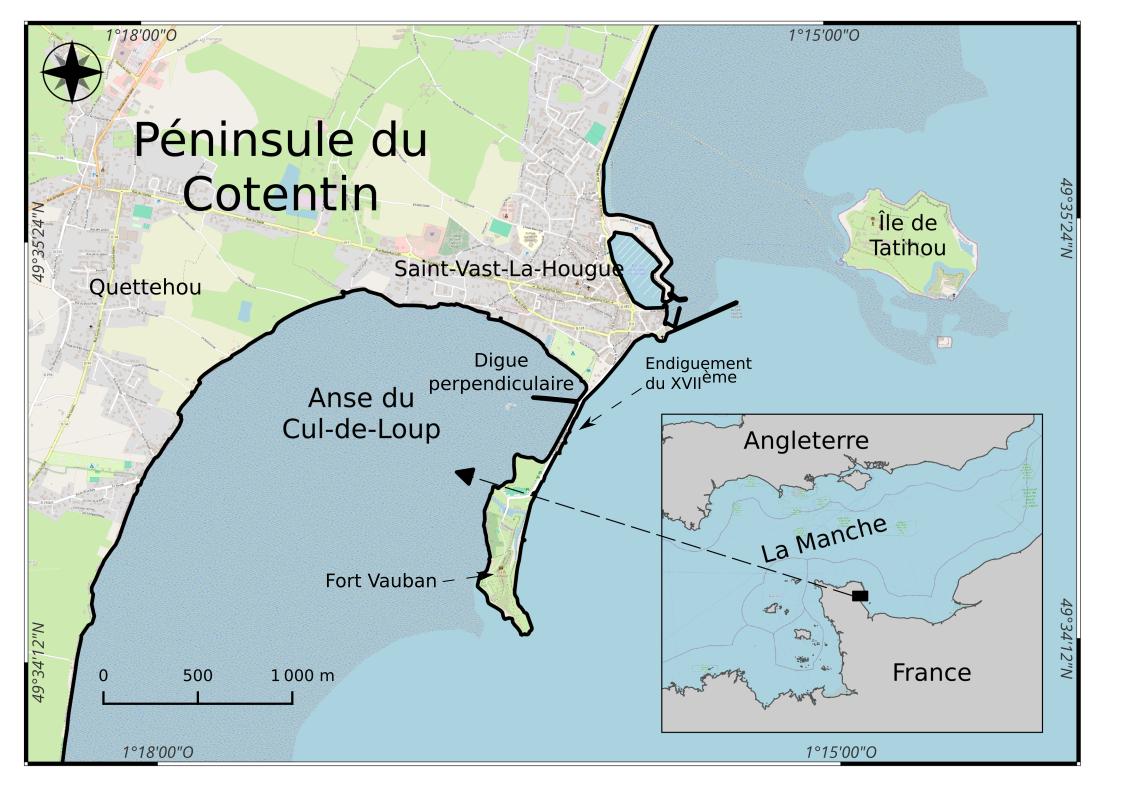
\includegraphics[width=0.8\linewidth]{../images/carte-ADCL}
        \caption[anse du Cul-de-Loup.]{L'anse du Cul-de-Loup.}
        \label{fig:carte-adcl}
    \end{figure}
    
    Le vent est régulièrement présent sur la zone du Cul-de-Loup, avec une moyenne de 18-19 km/h l'été majoritairement de secteur ouest et de 25-30 km/h en période hivernale avec un partage plus homogène des directions. L'agitation de surface dans l'anse est majoritairement de type mer du vent, due au frottement par le vent à la surface de l'eau.
    
    L'orientation de l'anse du Cul-de-Loup la protège des houles les plus fréquentes en Baie de Seine, qui sont de secteurs nord-ouest à nord-est essentiellement. Les houles de secteur est et sud-est sont les seules à éventuellement pouvoir pénétrer dans l'anse, mais elles sont à la fois plus rares et de faible énergie. Ces dernières sont rapidement dissipées par la présence des structures ostréicoles et pénètrent donc peu à l'intérieure de l'anse. A l'est au niveau de la bordure interne de l'Île de la Hougue, certaines houles peuvent néanmoins diffractées et être canalisées le long de l'île avec une énergie significative.
    
    \begin{figure}[!h]
        \centering
        \includegraphics[width=0.8\linewidth]{../images/historique}
        \caption[Évolution de l'anse du Cul-de-Loup]{En bas à gauche, image aérienne de 1942, l'anse du Cul-de-Loup ne contient aucun parc ostréicole. En bas à droite, image aérienne de 1965, l'anse du Cul-de-Loup commence à être aménagée dans sa partie nord. En haut à gauche et à droite, respectivement la morpho-bathymétrie  et une image aérienne actuelle de l'anse du Cul-de-Loup montrant de nombreuses concessions ostréicoles. (sourcer les images : géoportail)}
        \label{fig:historique-adcl}
    \end{figure}
    
    
    
    \newpage
    
    \section{MATÉRIELS ET MÉTHODES}
    \label{sec:materiel_methodes}
    
    \subsection{Le code de calcul CROCO}
    \label{sub:croco}
    %Mettre les principes généraux de CROCO (origine, type de modèle, etc...)
    Le modèle communautaire océanique côtier et régional (CROCO\footnote{CROCO : Coastal and Regional Ocean COmmunity model}) est une évolution du système de modélisation océanique régionale qui utilise une méthode adaptative de raffinement de grilles en Fortran (ROMS\footnote{ROMS : Regional Oceanic Modeling System}\_AGRIF\footnote{AGRIF : Adaptive Grid Refinement In Fortran}).
    Le code ROMS\_AGRIF a été développé jusqu'en 2014 par l'Institut de Recherche pour le Développement (IRD) et l'Institut National de Recherche en Informatique et en Automatique (INRIA). Ces organismes qui ont participé au développement du code CROCO avec
    l'Institut Français de Recherche pour l'Exploitation de la Mer (IFREMER),
    le Service hydrographique et océanographique de la Marine (SHOM),
    et le Centre National de la Recherche Scientifique (CNRS).
    L'aspect aujourd'hui communautaire de CROCO fédère à la fois les développeurs/utilisateurs de ROMS, ainsi que des universités et organismes étrangers tels que l'Université de Californie à Los Angeles (UCLA\footnote{UCLA : University of California, Los Angeles})
    et le département de Géophysique de l'université de Concepción au Chili (DGEO\footnote{DGEO : Departamento de Geofísica Universidad de Concepción, Chile}).
    
    % Le code et la documentation de ROMS\_AGRIF ont progressivement été modifiés pour devenir le modèle communautaire CROCO.
    
    Ce modèle CROCO permet désormais de réaliser des modélisations sur des grilles dont la résolution peut être de kilométrique (modèle régional) à métrique (modèle côtier).
    
    Le code CROCO est fondé sur la résolution des équations Navier-Stokes avec l'approche Reynolds Average Navier-Stokes (RANS) \alert{(ref*)}.
    %        [image possible sur les modèles possibles]}
Les modèles de la catégorie RANS permettent de mettre en \oe{}uvre des modélisations à des échelles spatiales et temporelles plus importantes que les approches Direct Numerical Simulation (DNS) ou encore Large Eddy Simulation (LES).

Le système d'équations de CROCO est flexible.
Il permet de choisir la méthode de résolution physico-chimique et de l'adapter à la configuration.
Les nouvelles fonctionnalités sont progressivement vérifiées par la communauté avec, le cas échéant, la mise en place de cas test afin d'en faciliter l'utilisation.


CROCO peut être exécuté sur les machines parallèles ou des clusters d'ordinateurs.
%permet d'activer la parallélisation des calculs effectués lors de la modélisation.
% Ainsi, pour certaines configurations, il est possible de modéliser des temporalités de l'ordre de l'année pour un coût de calcul abordable. (ex .)
Ainsi, en fonctions des objectifs, il est possible de mettre en place des modélisations à la fois finement résolues et couvrant des périodes de temps annuelles pour des coûts de calcul abordables.

%Enfin, en même temps que le développement du modèle, des outils communautaires de pré- et de post- traitement adaptés au fonctionnement de CROCO ont été développés.
Pour faciliter la mise en place des configurations CROCO, un ensemble d'outils ont été développés.
Ces outils ont d'abord été écrits en Matlab sous le nom de CROCO\_tools.
Plus récemment, de nouveaux outils développés en Python sont disponibles et appelés les CROCO Pytools.
% Le transfert des outils de Matlab vers Python renforce l'aspect leur ouvert et communautaires.
En éliminant la dépendance aux licences Matlab, ces nouveaux outils renforcent leur accessibilité et par conséquent leur universalité.

%+ Philosophie section (aspects spécifiques mis en oeuvre)
CROCO étant très polymorphe, une présentation de l'ensemble des caractéristiques offertes sort du contexte de ce travail.
Pour une description exhaustive de ces possibilités, une documentation est disponible et entretenue en ligne \cite{documentation_croco}.
%La nature et les possibilités accordées par CROCO sont très variées.
Dans la suite du rapport, seuls les aspects de CROCO spécifiquement utilisés pour la mise en \oe{}vre du Modèle de l'anse du Cul-de-Loup (MACLoup) sont présentés.


\subsubsection{Mise en \oe{}uvre de MACLoup}
\label{subsub:presentation_generale}
%\alert{[sous-section à reprendre + compléter, si possible, garder la relecture de cette partie pour plus tard] - A
    %    [ajouter la description des fichiers de configuration de croco (cppdefs, param.h, in, jobcomp)]}

La démarche générale de mise en place d'un modèle numérique hydrodynamique est relativement la même quelque soit les codes de calculs. Dans un premier temps, il faut définir et construire la représentation numérique du domaine modélisé. Dans un second temps, il faut définir les caractéristiques de la masse d'eau et la nature des écoulements qui vont être modélisés.

Si CROCO suit les mêmes principes généraux, il se distingue sensiblement sur ce dernier aspect. Il est issu du rassemblement de plusieurs codes de calcul qui avaient chacun leur propre philosophie de mise en place.  Ainsi, plusieurs fichiers de configurations doivent être construits en parallèle, contenant à la fois des informations propres, mais aussi, pour certains paramètres, des redondances qu'il est nécessaire de rendre homogène partout. C'est là une des principales difficulté dans la compréhension de mise en place d'un modèle avec CROCO à laquelle vient s'ajouter une documentation parfois sommaire ou partielle sur certaines parties du code (bien que des efforts soient engagés maintenant sur cet aspect). La figure \ref{fig:workflow_simple} résume les grandes étapes de l'établissement d'un modèle CROCO et les liens entre elles.

Concrètement, les fichiers de configurations sont toujours les mêmes quelque soit le modèle créé et sont au nombre de quatre (en bleu dur la figure \ref{fig:workflow_simple})~:
\begin{itemize}
    \item \textit{param.h}, est un fichier de paramètres qui indique les dimensions du maillage utilisé pour la modélisation ainsi que les variables associées à l'ensemble de la zone,
    \item \textit{cppdefs.h}, est un fichier qui définit essentiellement l'hydrodynamique du modèle, via des clefs de paramètres qui déterminent la manière dont le modèle interprète et propage les données. Il permet par exemple d'identifier quelles équations physiques doivent être résolues par le modèle,
    \item \textit{jobcom}, est un fichier exécutable qui contient les options de compilations du code CROCO, propres à l'environnement d’exécution,
    \item \textit{croco.in}, est un fichiers de paramètres qui défini, entres autres, l'étendue temporelle de la modélisation, les fréquences de sauvegardes des fichiers de sortie, ainsi que quelques valeurs constantes. Il donne aussi la localisation des données numérisant la zone.
\end{itemize}

Un schéma global de la mise en place du modèle est présenté en Figure \ref{fig:workflow_simple} \alert{nécessaire ? la figure a déjà été présentée plus tôt}
\begin{figure}[h!]
    \centering
    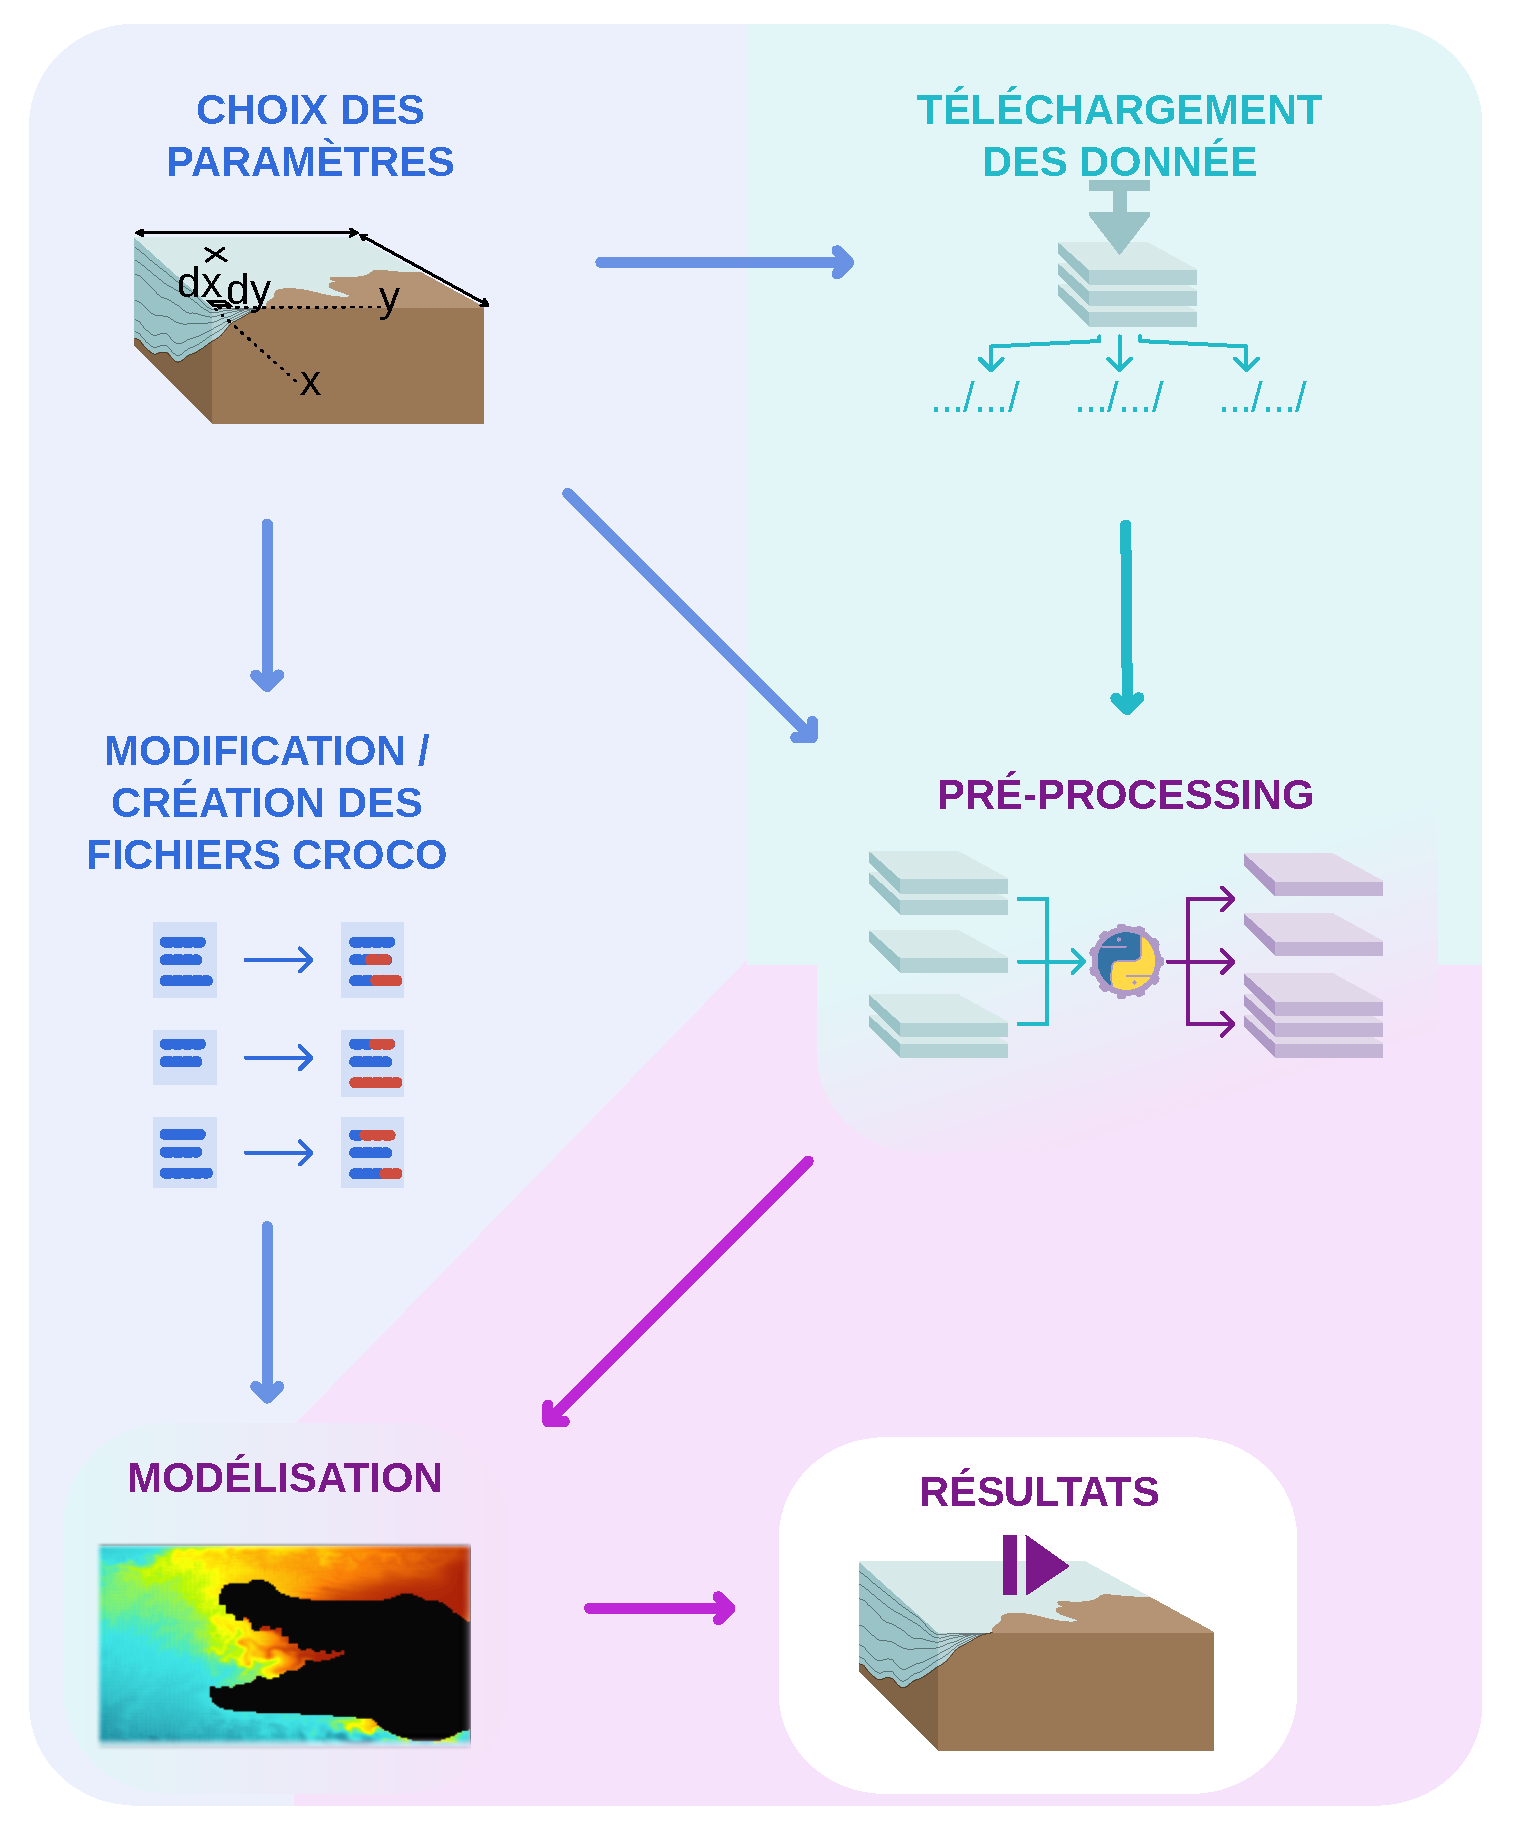
\includegraphics[scale=0.35]{../images/workflow/mise_en_place_generale_croco.pdf}
    \caption{\textbf{Mise en place du modèle CROCO avec une gille simple.}}
    \label{fig:workflow_simple}
\end{figure}

Les fichiers qui numérisent la zone étudiée, contiennent des données contraignant le déplacement des masses d'eau.
Ces fichiers sont intégralement à la charge de l'utilisateur·ice de CROCO.
Parmi ceux-ci, les forçages initiaux et aux limites, sont la source des mouvements de l'eau. Un autre fichier est celui qui définit la morphologie du domaine. Ce dernier est fondamental à la fois pour une retransmission la plus fidèle possible des écoulements fluides, mais aussi pour une bonne stabilité des calculs.

Les forçages peuvent contenir une large variété de données spatiales et temporelles.
On relèvera notamment la possibilité d'indiquer la valeur des températures, des salinités, des hauteurs d'eau relativement au niveau marins de référence, des vitesses de courant et des conditions atmosphériques à proximité de la surface.
Les données des forçages sont regroupées dans cinq principaux fichiers~:

\begin{itemize}
    \item le contexte morphologique du domaine modélisé (bathymétrie, limite côte-océan, etc.)(voir \ref{subsub:grille_croco});
    \item les phénomènes physiques qui forcent le déplacement de la masse d'eau (voir \ref{subsub:physique_modele})~:
    \begin{itemize}
        \item[.] la marée (amplitude et vitesse de déplacement des ondes de marée),
        \item[.] les conditions atmosphériques (vent, pluie, etc.),
    \end{itemize}
    \item les conditions physico-chimiques internes à la masse d'eau (voir \ref{subsub:forcages})~:
    \begin{itemize}
        \item[.] aux limites sur la période modélisées (température salinité, etc.),
        \item[.] sur l'ensemble de la zone modélisée à l'initialisation du modèle (temps $t_{0}$).
    \end{itemize}
\end{itemize}
%%%%%%%%%%%%%%%%%%%%%%%%%%%% FIN RELECTURE FUSION VERSIONS %%%%%%%%%%%%%%%%%%%%%%%%%%%%
Le contenu de ces fichiers doit respecter une structure et une nomenclature spécifique afin d'être utilisable par le code CROCO.
Il est généralement issu de l'extraction et de l'interpolation des données brutes par les outils communautaires associés à CROCO.

%Afin de simplifier le travail de pré-traitement, la communauté a développé des outils numériques de lecture, calcul et écriture de données.
%Ces codes de pré-traitement utilisent au choix des scripts Matlab (ces outils sont appelés croco\_tools) ou des scripts Python (ces outils sont appelés CROCO Pytools).
%L'utilisation dans le cadre du stage de ces outils est décrite dans la partie suivante.

\subsubsection{Le domaine MACLoup}
\label{subsub:grille_croco}

Le domaine CROCO, comme pour tout autre modélisation numérique, est une discrétisation spatiale de la morphologie réelle de la zone modélisée.
Il représente la bathymétrie et le trait de côte.
Le domaine est supporté par un maillage horizontal (2D) dont chaque n\oe{}ud est géoréférencé et présent au centre d'une maille.
Dans MACLoup, chaque maille suit la définition de \cite{Arakawa_C-grid_1977} en grille de type C.
Selon cette définition toutes les variables (température, salinité, hauteur d'eau, etc.) sont définies et résolues au centre des mailles ($H_{i,j}$, Figure \ref{fig:structure_maille horizontale}).
Seules les composantes $U$ et $V$ de la vitesse sont présentes aux bords des mailles (Figure \ref{fig:structure_maille horizontale}).
\begin{figure}[h!]
    \centering
    \begin{tabular}{ c c c }
        \multicolumn{1}{r}{·--} & $V_{i,{\color{red}j+1}}$ & \multicolumn{1}{l}{--·} \\
        | & & | \\
        | & & | \\
        $U_{i,j}$ & $H_{i,j}$ & $U_{{\color{red}i+1},j}$ \\
        | & & | \\
        | & & | \\
        \multicolumn{1}{r}{·--} & \textbf{$V_{i,j}$} & \multicolumn{1}{l}{--·}
    \end{tabular}
    \caption{
        Maille $i,j$ horizontale de type Arakawa C-grid.
        %Représentation d'une maille  du domaine CROCO.
        %Les tirets (\_|) indiquent les cotés de la maille.
        Les variables modélisées sont résolues en position $H_{i,j}$.
        Les composantes horizontales de vitesse sont présentes aux bords de la maille en position $U_{i,j}$ et $V_{i,j}$.
        %La position à laquelle est calculé chaque type paramètre de la maille est représentée par $U_{i,j}$, $V_{i,j}$ et .
        %La première lettre de ces indicateurs correspond au type des paramètres qu'elles représentent.
        Les composantes de vitesses $V_{i,j+1}$ et $U_{i+1,j}$ appartiennent aux mailles adjacentes.
        % suppose que la maille $i,j$ ne se situe pas à l'extrémité d'une ligne ou d'une colonne de son maillage.
        Cette représentation est issue de \cite{grid_doc}.
    }
    \label{fig:structure_maille horizontale}
\end{figure}


%La morphologie du domaine modélisé dans CROCO est présente sous la forme de maillages horizontaux et verticaux.
%Ce domaine est localisé en longitude et latitude à la surface de la Terre.
%Il contient trois maillages dont deux son issus de la translation Nord-Sud et Est-Ouest du maillage central sur une longueur d'une demi-maille.
%Pour chaque maille des trois maillages, une latitude et une longitude sont attribués dans le fichier du domaine CROCO.
%Le domaine contient aussi une donnée de bathymétrie / topographie pour chacune de ses mailles.
Pour séparer les zones immergeables des autres, un booléen est attribué à chaque maille, respectivement $1$ (True) pour les mailles immergeables et $0$ (False) pour les autres.
%Le domaine contient une donnée booléenne\footnote{valeurs indiquant soit \textit{vrai} (1) soit \textit{faux} (0)} attribuée à chaque maille du maillage principal.
%L'ensemble de ces données booléennes sont appelées le masque du domaine.
%Le masque indique quelles mailles sont définies comme toujours émergées.
Les équations ne seront jamais résolues au niveau des mailles non-immergeables du domaine.
%Le domaine CROCO est contenu dans un unique fichier NetCDF.

Le modèle MACLoup est défini en dimensions pseudo-3D, il est composé d'une succession de maillages 2D répartis verticalement selon une dimension $\sigma$.
Dans cette définition, les couches sont contraintes verticalement par la bathymétrie et réparties analytiquement sur la hauteur de la colonne d'eau.
Par convention, la surface est à $0$ et le fond est à $1$ sur la dimension $\sigma$.
Cette répartition est modulée selon deux paramètres $\sigma_{s}$ et $\sigma_{b}$ qui décrivent la résolution verticale respectivement à l'approche de la surface et du fond (Fig. \ref{fig:vertical_resolution}).
%La résolution verticale du maillage n'est pas définie dans le fichier du domaine CROCO.
Cette paramétrisation de la verticale est indiquée dans les fichiers d'entrées \textit{param.h} et \textit{croco.in} de la configuration.
%Selon les paramètre choisis, la résolution verticale peut varier verticalement selon les deux paramètres $\sigma_{s}$ et $\sigma_{b}$.
%Ces derniers décrivent le taux d'augmentation ou de diminution de la résolution verticale respectivement à l'approche de la surface et du fond.

[indiquer l'existence du masque de côte]

\begin{figure}[h!]
    \centering
    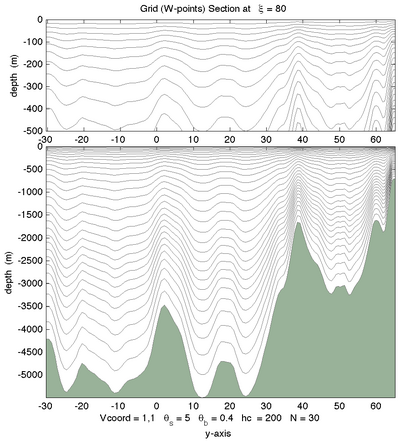
\includegraphics[scale=0.7]{../images/vcoord_ex1.png}
    \hspace{2cm}
    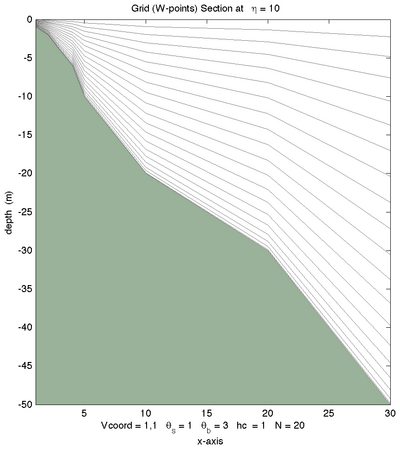
\includegraphics[scale=0.7]{../images/vcoord_ex5.png}
    \caption{\textbf{Exemples de résolutions verticales variables déterminées par la topographie et les paramètres  $\sigma_{param}$ entrés par l'utilisateur·ice.} \\
        À gauche, les paramètres choisis sont  $\protect\theta_s = 7$, $\protect\theta_b = 0,1$, à droite ils sont  $\protect\theta_s$ = 7, $\protect\theta_b = 3$.
        Ces figures proviennent de la documentation CROCO \cite{grid_doc} et ont été fournies par l'équipe ROMS-RUTGERS}
    % (source : https://croco-ocean.gitlabpages.inria.fr/, https://myroms.org/)
    \label{fig:vertical_resolution}
\end{figure}

%Les variables physico-chimiques que le modèle propage ont généralement un effet rétroactifs sur leur propre propagation ou-et sur la propagation d'autres variables.

\subsubsection{Hydrodynamique de MACLoup}
\label{subsub:physique_modele}
C'est le fichier nommé \textit{cppdefs.h} (Fig. \ref{fig:workflow_simple}) qui détermine les caractéristiques hydrodynamiques effectivement résolues dans le modèle.
% quelles équations physiques doivent être résolues par le modèle.
La définition de ces caractéristiques s'appuie sur la présence de mots clefs.
Chaque mot clef active ou désactive une fonctionnalité avec la syntaxe "\# define"  ou "\# undef" qui le précède.
Par exemple, l'ajout de la ligne "\# define SALINITY" dans \textit{cppedefs.h} active, au moment de la compilation, la prise en compte de la salinité.


%Dans le cadre du stage, le contenu du fichier a été défini pour que les équations résolues prennent la forme d'un schéma d'advection de cinquième ordre WENO5 (Annexes \ref{anx:WENO}) et d'un schéma de diffusion adapté à la configuration.
%Une précision des choix effectués est donné dans l'encadré suivant \ref{encadre:precisions_schema}.

%\begin{codeEnv}{Les schémas d'advection et de diffusion\label{encadre:precisions_schema}}
%(\cite{dev_RANS-LES_these}, \cite{comp_RANS_LES})
%Les équations utilisées et résolues par CROCO durant la modélisation sont flexibles.
Les premiers choix fondamentaux à faire sont ceux des types de schémas numériques de résolution de l'advection et de la diffusion.
Le code CROCO propose divers schémas qu'il est nécessaire de choisir en cohérence. % (entre eux)
%[enlever ?]
%Les schémas numériques possibles pour l'advection sont au minimum de second ordre et au maximum de cinquième ordre.
%Les schémas numérique de diffusion sont laplaciens ou biliplaciens. (ça se dit probablement autrement !)
%[]
%Le choix des schémas est libre pour l'utilisateur·ice, (\cite{schemas_advection}) il est toutefois important de noter que les schémas choisis doivent être cohérents entre eux.
Certains schémas sont mieux adaptés que d'autres à chaque configuration.
Il est donc important que cette dernière soit correctement identifiée avant de choisir les schémas numériques.

Dans l'anse du Cul-de-Loup, la côte est tortueuse et de larges zones sont régulièrement découvertes et recouvertes au cours d'un cycle de marée.
D'un point de vue numérique, ces caractéristiques sont contraignantes et déterminent la nature des schémas d'advection possibles.
%Dans MACLoup, le nombre de couches verticales est faible ($\leq 30$) et la topographie est assez découpée par endroits.
Ces choix ont principalement faits sur la base de la documentation principale \parencite{cppkeys_description}.
Ils ont été complétés avec la configuration du modèle de plage de  \cite{swash_article_MARCHESIELLO2021101816}.
Ce dernier modèle fait face à des dynamiques de découvrement régulier de certaines mailles de la grille dans la zone d'action des vagues.
Cette dynamique est analogue à celle de notre configuration.
%En effet, dans le modèle de l'anse du Cul-de-Loup, le découvrement s'effectue sur les mailles dans la zone de balancement des marées.
%La même robustesse que la configuration précédemment citée est donc recherchée.

Le schéma retenu est celui d'advection quasi-monotone de cinquième ordre de WENO\footnote{Weighted Essentially Non-Oscillatory scheme} (voir Annexes \ref{anx:WENO}).

Le choix du schéma numérique de diffusion est de type Generic Length Scale (GLS).
Les schémas de diffusion verticale et horizontal sont différenciés.
En effet, les résolutions verticales et horizontales sont différentes (voir section \ref{subsub:grille_croco}).
%Le schéma vertical est conditionné par la structure de la grille du modèle.
%Dans la configuration MACLoup, les couches horizontales de la grille sont d'épaisseur variables et suivent la topographie.
Le schéma de diffusion horizontale choisi est de type Laplacien avec une viscosité turbulente paramétrisée avec la méthode de Smagorinsky (\cite{schemas_diffusion_horizontale}).
Enfin, le schéma de diffusion horizontale est de type K-OMEGA provenant de \cite{GLS_KOMEGA_kolmogorov1941equations}.
%\end{codeEnv}

L'ensemble des clefs activées qui définissent le schéma d'advection-diffusion de MACLoup se trouve en Annexes (Section \ref{anx:cppdefs}).


\subsubsection{Les forçages du modèle}
\label{subsub:forcages}
%L'ensemble de des paramètres et variables donnés par l'utilisateur définissent les forçages physico-chimiques imposés au modèle.
On entend par forçages les phénomènes et les forces primaires qui mettent directement en mouvement la masse d'eau.
Les principales forces sont la marée, le vent et la gravité.
La présentation de ces forces est restreinte à celles qui sont utilisées dans le cadre de notre étude.
Concrètement, dans CROCO, les forçages sont regroupés dans plusieurs fichiers selon le moment et le lieu où ils s'appliquent dans le modèle.
%Les données des forçages sont au format NetCDF.

L'hydrodynamique de l'anse du Cul-de-Loup est dominée par les forces de marée.
La marée est donc le forçage principal de MACLoup et fait l'objet de la construction spécifique d'un fichier.
%d'inclure les données tidales dans un fichier de forçage.
%La troisième catégorie correspond aux forçages de marée.
%Ces derniers remplacent les données de hauteur d'eau et éventuellement de courant des conditions aux bordures.
Ce fichier, \textit{croco\_frc.nc}, contient $n$ harmoniques de marée pour lesquelles sont indiquées les amplitudes et les phases des hauteurs d'eau. Il peut contenir en plus les deux composantes horizontales de la vitesse de déplacement de l'onde de marée.

Il est nécessaire, au démarrage du modèle ($t_0$), que les conditions environnementales (Température, salinité, vitesse du vent et de l'eau) soient les plus proches possible des conditions réelles à la date à laquelle le modèle doit démarrer.
%que la modélisation soit initialisée avec des variables qui représentent au mieux les conditions réelles au départ du modèle.
%La seconde catégorie correspond aux forçages qui définissent les conditions initiales.
Un fichier de forçage est donc attribué à ces conditions initiales.
Ce fichier, \textit{croco\_ini.nc}, contient notamment les données de température, salinité, hauteur d'eau et vitesses des courants sur l'ensemble du maillage à l'initialisation du modèle.

Le domaine modélisé étant spatialement fini, il est nécessaire que des conditions aux bords soient données.
Les valeurs aux bords complètent celles contenues dans les forçages de marée.
%latéraux du domaine des variables qui ne sont pas définies dans les forçages de marée sont définies dans un troisième fichier de forçage.
%La seconde catégorie correspond aux forçages qui définissent les conditions aux bords latéraux de la grille.
Ce fichier, \textit{croco\_bry.nc}, contient notamment les données de température et de salinité %et éventuellement hauteur d'eau et vitesses des courants
aux bords de la grille sur toute la durée temporelle de la modélisation.


Des conditions atmosphériques peuvent être ajoutées aux forçages déjà présents afin de mieux approcher la réalité lors de la modélisation.
%La quatrième catégorie correspond aux forçages atmosphériques.
Un fichier supplémentaire, \textit{croco\_blk.nc}, est construit, il contient notamment l'humidité, la température, la pression de l'air au dessus de la surface de l'eau, la vitesse du vent à $10~m$ au dessus de la surface, des paramètres sur les contraintes de surfaces imposés par le vent et les radiations solaires reçues par la masse d'eau pour les courtes et longues longueurs d'ondes.
Ces informations sont données sur toute l'étendue du maillage horizontal sur toute la durée temporelle de la modélisation.

\subsubsection{Modélisation par emboîtement de domaines}
\label{subsub:enchainement_modelisations}
%Le modèle CROCO permet de mettre en place l'étude d'un lieux en réalisant plusieurs modélisations.

Les conditions initiales et aux limites ne sont pas toujours suffisamment précises pour permettre de démarrer directement le modèle sur le domaine d'intérêt.
Le principe est de générer ces conditions avec un premier domaine adapté aux données disponibles.
Les résultats de cette première modélisation sont utilisés comme données initiales sur le domaine d'intérêt.
Il est donc nécessaire que le domaine d'intérêt (domaine enfant) soit intégralement contenu (emboîté) dans le domaine initial (domaine parent).

%Cette méthode d'emboîtement de domaines permet de s'affranchir du besoin de données externes pour les conditions aux bords du domaine d'intérêt qui est le moins étendu et qui est le mieux résolu.
L'objectif de la démarche est d'obtenir des résultats qui convergent plus vite vers des données justes pour un coût de modélisation soutenable.

%L'usage principal de cette fonctionnalité consiste à emboîter plusieurs domaines de résolution croissante et d'étendue décroissante autour d'un zone d'intérêt.
Il est possible de généraliser la démarche sur une suite de domaines successivement emboîtés.
%Un domaine A contenant un domaine B est appelé le domaine parent du domaine B.
%Le domaine B est appelé le domaine enfant du modèle A.
Tous les domaines enfants extraient leur conditions aux limites des résultats de leur domaine parent respectif.

Dans CROCO, il existe deux manières de prendre en charge un système en domaines emboîtés : un emboîtement de type temps-réel et l'autre de type temps-différé.
La méthode de type temps-réel est prise en charge dans CROCO via le module spécifique AGRIF\footnote{AGRIF : Adaptive Grid Refinement In Fortran}.
Cette méthode n'a pas été retenue dans le cadre de MACLoup, des précisions sur ce point sont présentes en Annexes (\ref{anx:AGRIF}).
Le choix de la méthode d'emboîtement s'est donc porté sur le type temps-différé.
Dans ce mode, Les modèles sont exécutés les uns après les autres en commençant par le domaine parent de plus haut niveau.
Les résultats de chaque parent sont successivement utilisés pour générer les fichiers de forçages du domaine sous-jacent.

Cette méthode est illustrée en \ref{fig:imbrication_workflow} et \ref{fig:imbrication}.

\begin{figure}[h!]
    \centering
    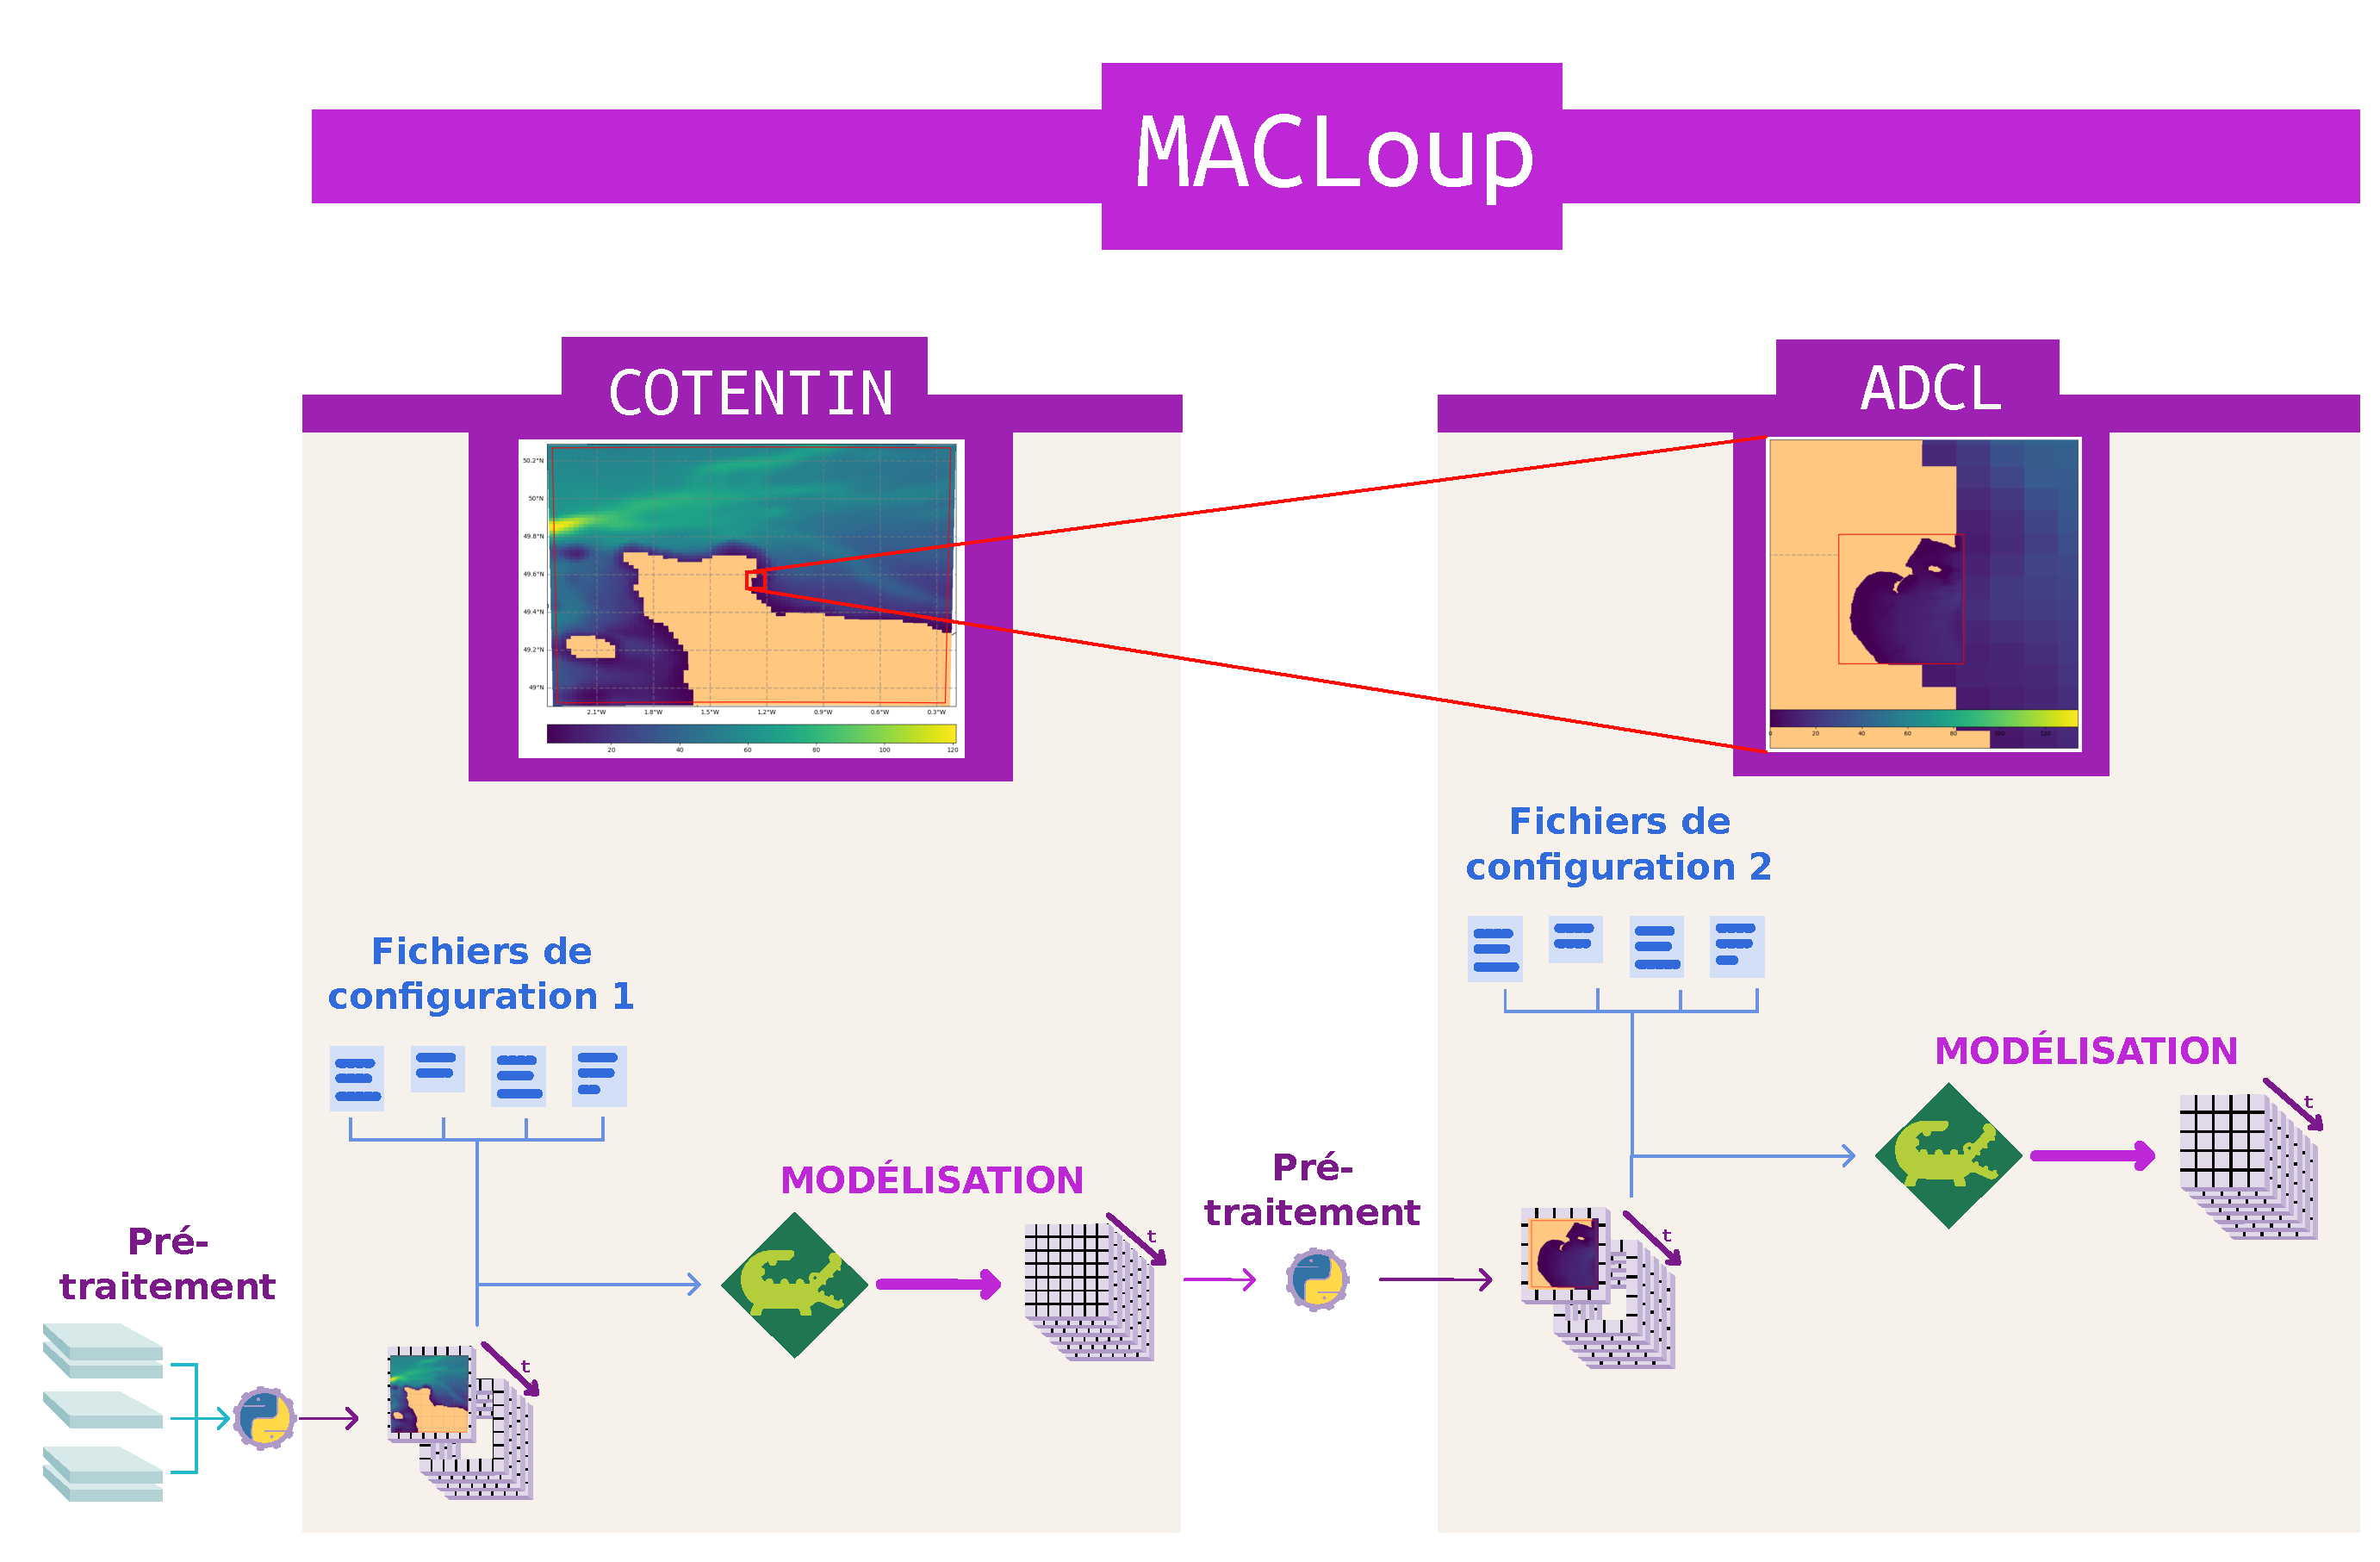
\includegraphics[scale=0.3]{../images/workflow/multi_grid.pdf}
    \caption{Schéma de la mise en place des domaines emboîtés du modèle MACLoup. Les étapes peuvent être répétées pour }
    \label{fig:imbrication_workflow}
\end{figure}

Dans le cadre de MACLoup, deux domaines successifs sont modélisés.
Le premier domaine couvre une zone de $150$ par $150~km$ centré sur le département de la Manche.
Le second est centré sur l'anse du Cul-de-Loup, sur une zone de $7$ par $11~km$ (Figure \ref{fig:imbrication}).

%La zone d'intérêt de MACLoup est fortement restreinte dans l'espace et les données doivent y être finement modélisées.
%Une démarche d'emboîtement de domaines a donc été mise en place pour la modélisation de l'anse du Cul-de-Loup (MACLoup).


\begin{figure}[h!]
    \centering
    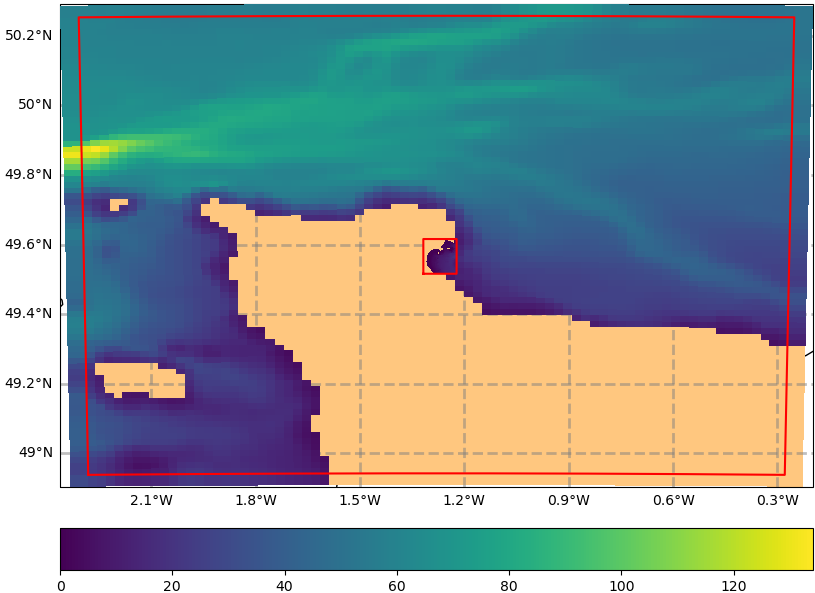
\includegraphics[scale=0.4]{../images/COTENTIN_ADCL5.png}
    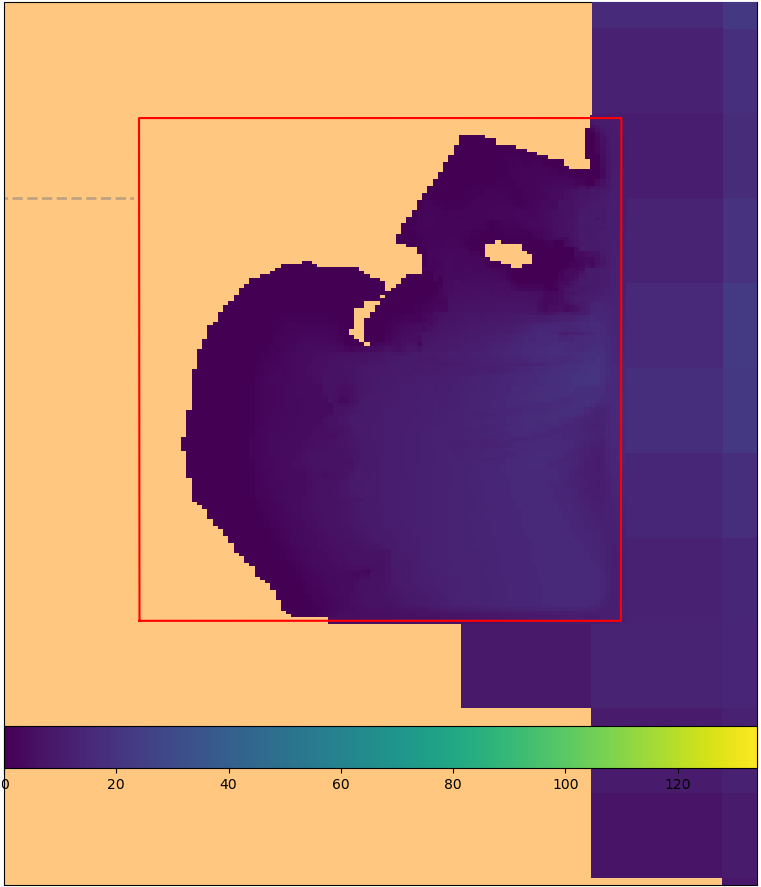
\includegraphics[scale=0.27]{../images/ADCL5.png}
    %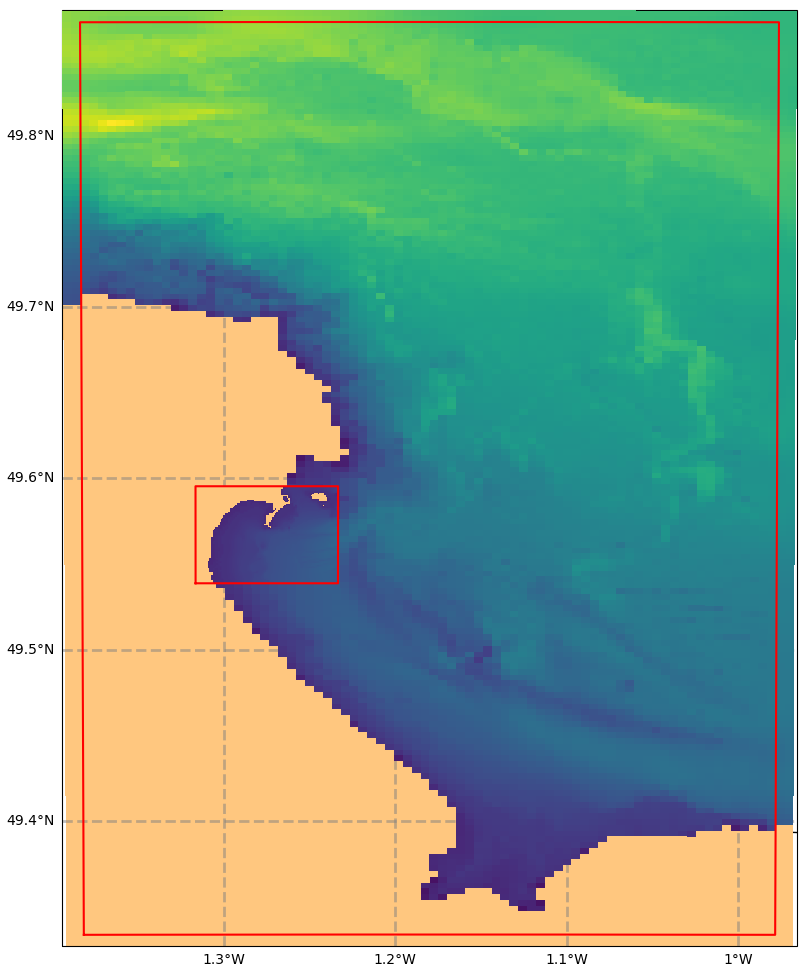
\includegraphics[scale=0.27]{../images/croco_grd.nc.2_V2.png}
    \caption{
        \textbf{Visualisation des domaines emboîtés choisis pour MACLoup.}\\
        \textbf{À gauche}, le grand rectangle rouge représente l'empâtement le domaine parent, le petit rectangle représente le domaine cible.
        \textbf{À droite}, une capture plus recentrée sur le domaine cible.
        Les données à l'extérieur du rectangle correspondent au domaine parent.
        \\
        Pour les deux figures, les pixels oranges sont les maille considérées comme obligatoirement émergées.
        Les autres couleurs (du bleu au jaune) représentent la bathymétrie dont les échelles respectives sont représentées en dessous de chaque graphique.
    }
    \label{fig:imbrication}
\end{figure}

%Un autre usage de modélisation sur plusieurs grilles en parallèle (AGRIF) consiste à mettre en continuité spatiale des grilles de même résolution afin de modéliser une zone dont la forme n'est que peu similaire à celle d'un rectangle.
%Cet usage est en particulier proposé pour effectuer une modélisation le long d'un trait de côte sinueux.
%Ainsi, moins de données brutes pour les conditions aux limites sont nécessaires par rapport à une modélisation de multiples grilles de manière indépendante.
%Cet usage ne correspond pas aux besoin de cette étude qui a pour but de modéliser une zone aisément assimilable à un rectangle, c'est à dire que cette zone peut être efficacement représentée par une unique sous-grille.

\subsection{Les outils de pré-traitement}
\label{sub:outils_pretraitement}

Le pré-traitement correspond à la création des fichiers nécessaires au démarrage de CROCO.
Il inclue :
\begin{itemize}
    \item la création du domaine qui représente la zone modélisé (voir \ref{subsub:grille_croco}),
    \item la création des différents forçages (voir \ref{subsub:forcages}).
\end{itemize}

Dans le cadre du stage, ce sont les CROCO Pytools qui sont utilisés pour ce travail.
%Ces outils sont identifiés comme les \textit{CROCO Pytools} et sont ceux qui ont été intégrés dans l'univers CROCO le plus récemment.

Les CROCO Pytools sont encore en cours de développement. %, les utiliser permet de participer à la vérification de leur fonctionnement par la communauté.
Certaines fonctionnalités sont encore à valider ou à développer.

%Il est donc nécessaire de les ajouter soit en modifiant les scripts déjà présents, soit d'écrire des scripts supplémentaires pour réaliser certaines tâches spécifiques.

%\begin{itemize}
%\item création de la grille de calcul (grille CROCO) décrivant la morphologie du domaine modélisé avec %\textit{make\_grid.py};
%\item création des conditions aux bordures du domaine modélisé avec \textit{make\_bry.py} ou %\textit{make\_zoom\_ibc.py};
%\item création des conditions initiales à l'intérieur du domaine modélisé avec \textit{make\_ini.py} ou %\textit{make\_zoom\_ibc.py};
%\item création des conditions de forçages pour la mise en mouvement de la masse d'eau avec %\textit{make\_frc.py} et \textit{make\_blk.py}.
%\end{itemize}

%\subsubsection{Modifications et apports aux CROCO Pytools}
L'ensemble des travaux associés au prétraitement représentent le c\oe{}ur du travail effectué durant le stage.
Ces travaux sont structurés en trois parties principales :
\begin{itemize}
    \item un état des lieux des outils existants et de leur fonctionnement général,
    \item une utilisation directe des CROCO Pytools en apportant, si nécessaire, des modifications,
    \item le développement d'outils manquants.
\end{itemize}

\subsubsection{État des lieux}
\label{subsub:etat_des_lieux}

Dans un premier temps, l'état des lieux des CROCO Pytools a été dressé.
Ce travail a abouti à une synthèse des outils présents et de la marche à suivre pour leur mise en \oe{}uvre (Fig. \ref{fig:workflow_prepro_original}).

\alert{[texte sur la figure de synthèse]
    [+ indication de la version plus complexe en annexes]}
\begin{figure}[h!]
    \centering
    %\includegraphics{}
    \caption{
        \textbf{[FIGURE À FAIRE]}
        version similaire à la Figure \ref{fig:workflow_prepro_main}
    }
    \label{fig:workflow_prepro_original}
\end{figure}


\subsubsection{Modification et utilisation}

Parmi les CROCO Pytools, quatre outils ont été utilisés et mis en \oe{uvre} moyennant des modifications sensibles.
% pour la création du domaine et de ses conditions initiales et aux bords.
%Au préalable, les dysfonctionnalités des codes ont été recherchées.

Le premier code, \textit{make\_grid.py}, permet de créer les domaines CROCO.
Il prend en charge la création du masque qui sépare les mailles émergées des mailles immergeables.
Cette opération utilise un fichier de données vectorielles représentant le trait de côte.
La version de l'outil ne fonctionne pas avec le fichier qui lui a été fourni pour créer le domaine MACLoup.
La solution adoptée consiste à modifier les données de bathymétrie en imposant une valeur forte et aberrantes  aux mailles émergées.
% ne prend pas en compte nos données vectorielles .shp pour déterminer le masquage des mailles non-immergeables.
%Toutefois, la fonctionnalité de seuillage des données de bathymétrie est fonctionnelle.
%Le masque du domaine a donc été imposé en fixant les données de bathymétrie des zones émergées au dessus du seuil choisi.
Cette modification des données rend inadaptée la procédure de lissage préexistante.
Cette dernière a nécessité d'être redéfinie de manière à ne pas être influencée par les données des mailles émergées.
%Cette modification a soulevé un autre problème du code de création du domaine.
%En effet, le code permet de choisir une distance d'interpolation plus ou moins grande et les valeurs sélectionnées pour l'interpolation peuvent être localisées sous le masque.
%Pour éviter que les données modifiées appartenant au masque n'aient une influence sur les données de bathymétrie, l'option d'interpolation n'a pas été utilisée pour le domaine d'intérêt centré sur l'anse du Cul-de-Loup.
Le code \textit{make\_grid.py} gère aussi la mise en place de domaines emboîtés qu'il s'agisse du type temps réel (AGRIF) ou du type temps-différé (notre choix) décrits en section \ref{subsub:enchainement_modelisations}.
%La première méthode permet de mettre en place le système d'esmboîtement de domaines simultané et rétrospectif.
%Cette méthode de création de domaines emboîtés est appelée AGRIF dans les CROCO Pytools.
%La seconde méthode permet de mettre en place manuellement et successivement un emboîtement linéaire de domaines.
%Cette méthode est appelée Offline Zoom, le système d'emboîtement qu'elle génère est décrit à la suite du système AGRIF en section \ref{subsub:enchainement_modelisations}.
%La méthode AGRIF de création de domaines emboîtés a été testée dans un premier temps.
%Il est apparu que son implémentation dans les CROCO Pytools est encore incomplète.
%D'autre part, l'utilisation du système d'emboîtement AGRIF impose des dépendances sur les clefs définies dans le fichier \textit{cppdefs.h} (section \ref{subsub:physique_modele}) activées pour la modélisation.
%[vérifier la véracité de cette phrase]
La procédure d'emboitement de type temps-différé est identifiée comme "Offline Zoom" dans l'outil
%qui est utilisée pour la génération des domaines emboîtés présentés dans la suite du rapport.
et a été utilisée sans adaptation particulière.
%et n'implique pas de dépendances particulières pour les clefs du fichier \textit{cppdefs.h}.
%[ajouter qu'on a des doutes du la prise en charge du wet/dry ? => non, a l'air ok en regardant les nouvelles grilles (ou effet vite dissipé d'une fine tranche d'eau initiale)]

Les deux codes \textit{make\_bry.py} et \textit{make\_ini.py} sont chargés respectivement de la création des données au bords et des conditions initiales du domaine.
Des modifications leur ont été apportées afin qu'ils prennent en charge la structure et le format des données brutes utilisées pour MACLoup.
%Par ailleurs, le code de création des conditions aux bords présente des dysfontionnalités qui semblent internent.
%Elles ont été résolues en modifiant un module des CROCO Pytools que ce code utilise.

Dans le cadre d'un emboîtement de domaine, le dernier outil, \textit{make\_zoom\_ibc.py}, permet la création de conditions aux bords et initiales héritées d'un modèle parent.
Cet outils s'est révélé fonctionnel sans que des modifications importantes n'y soient apportées.


%%%%%%% AJOUT à gérer %%%%%%%%%%ù


%Comme décrit en \ref{subsub:forcages}, chaque domaine CROCO, pour être utilisée par le modèle, doit être accompagnée par d'autres fichiers de forçages qui contraignent l'initialisation et la mise en mouvement de la masse d'eau.

%Les outils de pré-traitement originaux n'ont été utilisés que pour la génération du domaine et des conditions initiales et aux limites des grilles.





%\textbf{Le domaines CROCO}\\
%Pour le domaine parent comme pour les domaines enfants, le fichier définissant le domaine, "croco\_grd.nc", est généré avec le script \textit{make\_grid.py} des CROCO Pytools.
%\\
%Toutefois, cette fonctionnalité des CROCO Pytools ne semble pas encore fonctionnelle.
%Les données vectorielles du trait de côte sont donc corrigées par les données des campagnes plus précises mais qui couvrent seulement le Nord du Cotentin.

%Pour les domaines enfant, le fichier "croco\_ini.nc" est généré avec le script \textit{make\_zoom\_icb.py}.
%Les données utilisées sont les sorties de modélisations des domaines parents.

%Pour les domaines enfant, le fichier "croco\_bry.nc" est généré en même temps et avec les mêmes données que le fichier "croco\_ini.nc" avec le script \textit{make\_zoom\_icb.py}.



\subsubsection{Outils développés}

Comme expliqué en Section \ref{subsub:forcages}, les phénomènes de marée sont centraux dans l'hydrodynamique de l'anse du Cul-de-Loup.
Une attention particulière a donc été portée sur le choix du modèle de marée utilisé.
Le modèle TPXO10 est le modèle traditionnellement utilisé.
Il apparaît de plus en plus dans la littérature scientifique que le modèle Finite Element Solution (FES2014) lui est préféré.
Une nouvelle version du modèle de marée FES (FES2022) est disponible depuis peu mais ne contient pas les données de vitesse de l'onde de marée.
Le modèle FES2014 a été choisi car il est préférable pour la qualité et la performance des calculs que ces vitesses soient présentes dans les données de forçages plutôt que d'être définies analytiquement.
%Nous avons sélectionné la version FES2014 car elle contient les données de courants et de hauteur d'eau à l'inverse de FES2022 qui ne contient pour l'instant que les données de hauteur d'eau.
%Si les données de FES2022 sont complétées dans le futur, il sera alors possible d'aisément re-modéliser les domaines avec les nouvelles données.

La différence majeure entre les deux modèles TPXO10 et FES2014 réside dans le nombre d'harmoniques de marée qu'ils contiennent.
Le modèle FES2014 en contient 33 tandis que TPXO10 en propose 15.
Deux modélisations test ont été réalisées pour vérifier l'effet des 18 harmoniques supplémentaires de FES2014 en sortie de modélisation.
Les résultats sont présentés en Figure \ref{fig:ana_freq_cotentin}.

\begin{figure}[h!]
    \centering
    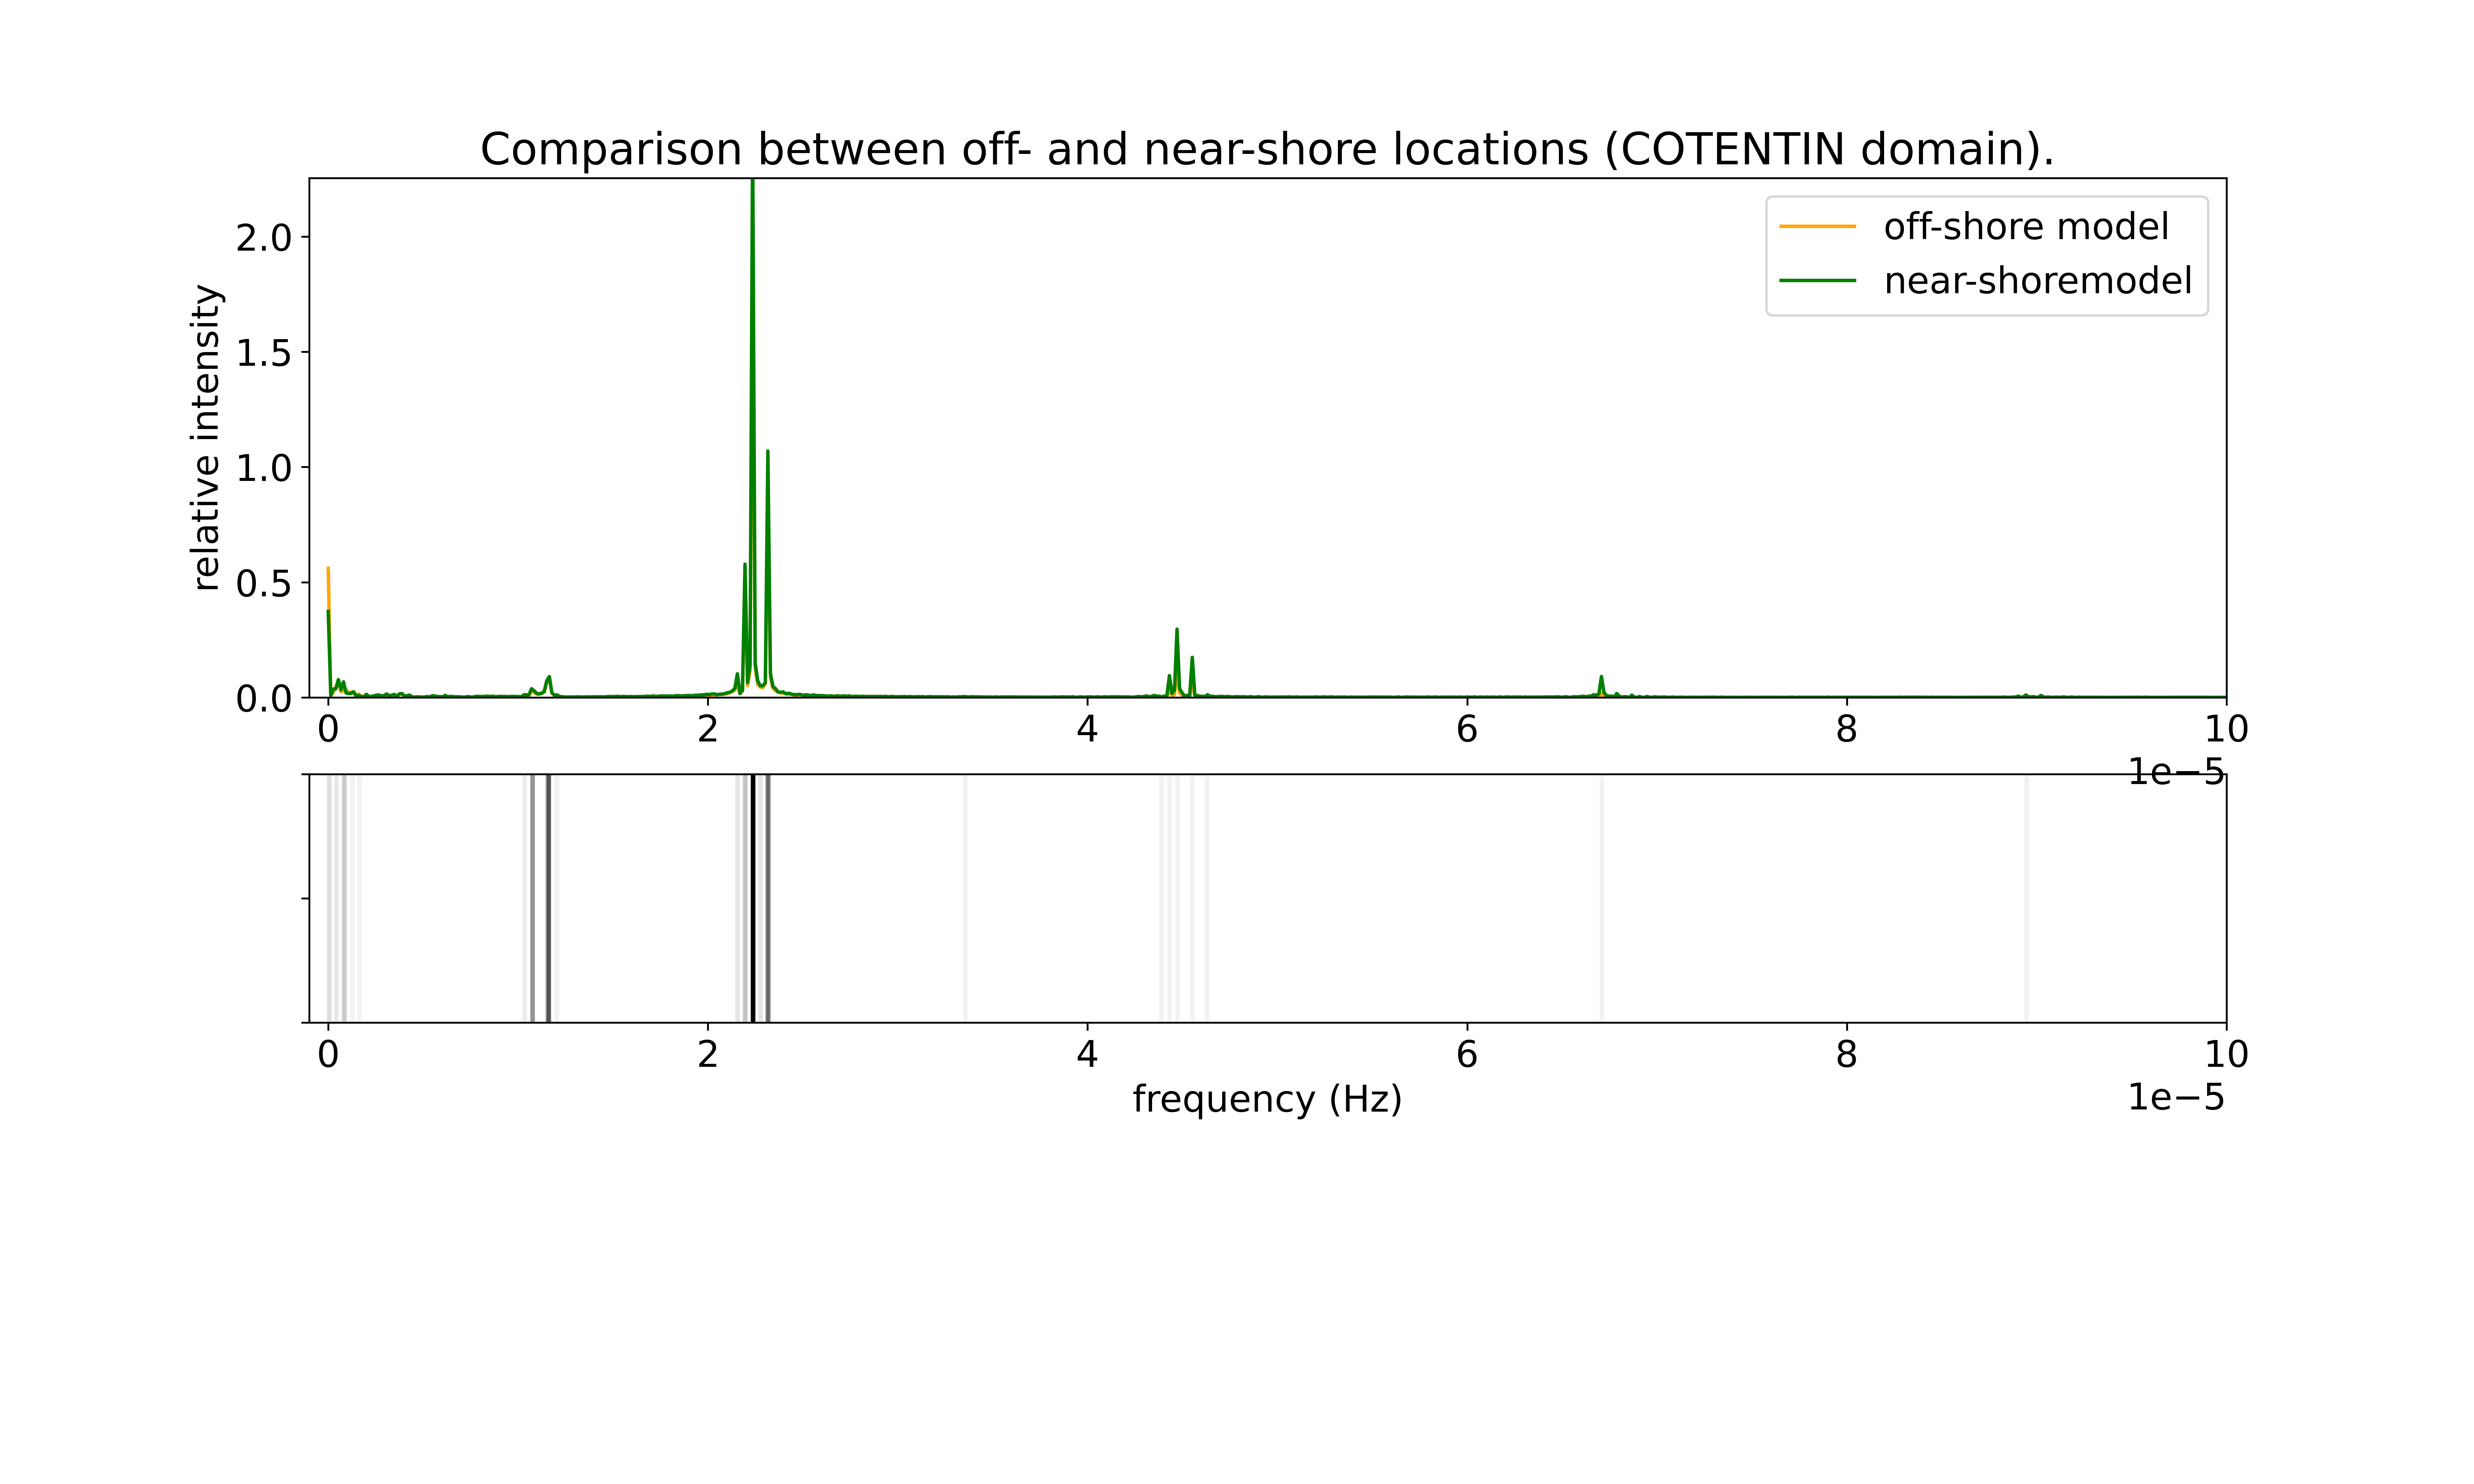
\includegraphics[scale=0.4]{../images/COTENTIN_analyse_off-near-shore.png}
    \caption{
        Analyse fréquentielle des données de sortie de la première phase de modélisation à large échelle (pour la méthode, voir \ref{sub:postpro}).
    }
    \label{fig:ana_freq_cotentin}
\end{figure}

\alert{[à compléter (analyser) avec la figure]}
Il apparaît qu'il est intéressant de prendre en compte des harmoniques supplémentaires à celles de TPXO10 en utilisant les données de FES2014.
%\alert{Le modèle FES2014 a été édité en 2014 son intégration dans les CROCO Pytools est récente.}
Étant donné l'importance du forçage tidal, il a été choisi de développer un outil dont le contenu et les opérations sont maîtrisés et explicites.
%Les codes de création des forçages de marée et atmosphériques des CROCO Pytools n'ont pas été fonctionnels avec les données utilisées dans le cadre du stage.
%L'écriture de ce nouvel outil a été dictée par les exemples de résultats offerts par les CROCO tools (en Matlab) disponibles en ligne \parencite{croco_files_examples}.
La démarche adoptée est de type rétro-ingénierie, par analyse des résultats issus de l'utilisation des CROCO tools (en Matlab) disponibles en ligne \parencite{croco_files_examples}.
Le code de ce nouvel outil a été développé pour une utilisation générique au regard des différents formats des jeux de données utilisés.
%dans le but de pouvoir être appliqué à des données dont les nomenclatures varient en permettant à l'utilisateur·ice d'adapter une entête aisément par l'intermédiaire de dictionnaires.
%Des tests sont encore nécessaires pour s'assurer du bon fonctionnement de cette option.
En outre, le développement de l'outil a permis de proposer une nouvelle approche d'interpolation en la rendant paramétrable, ce qui permet de l'adapter au jeu de données utilisé et aux conditions de la zone modélisée.
%Les processus réalisés par l'outil reposent sur la mise en place d'une interpolation paramétrable des données du modèle entrée afin de générer un fichier de forçage correspondant au domaine créé par l'utilisateur·ice.
%Pour que les forçages tidaux soient correctement interprété par CROCO certaines variables du modèles doivent être traduites.
%Cette transformation est implémentée dans le code original des CROCO Pytools.
%Les calculs ont donc été mis en place de la même manière que dans l'outil original en suivant définition de \cite{ap2ep}, les détail de ces calculs est donnée en Annexes \ref{anx:ap2ep}.

Les données de forçage atmosphérique sont contenues dans un fichier nommé \textit{croco\_blk.nc}.
Aucun outils n'est jusqu'alors présent dans les CROCO Pytools pour générer ce fichier.
Un nouvel outil a donc été développé en reprenant la démarche rétro-ingénierie et l'objectif d'utilisation générique des jeux de données.
Ce nouvel outil a été nommé \textit{make\_blk.py}.

Pour que les processus effectués par ces deux nouveaux codes de créations des fichiers de forçages soient mis en commun et organisés, quatre modules et classes ont été écrits~:
\begin{itemize}
    \item la classe "Operators" contient quelques fonctionnalités élémentaires comme l'affichage d'une erreur ou d'un dictionnaire, la gestion du type de certaines données (entiers, chaînes de caractères, tableaux, listes numpy) et le calcul d'un interpolation linéaire.
    La classe "Operators" n'est pas instanciée dans les codes de pré-traitement écrits.
    Ses fonctionnalités sont uniquement  utilisées par héritage par deux autres classes "NcFiles" et "Grid",
    \item la classe "NcFile" hérite de la classe "Operators" et ajoute des fonctionnalités de lecture et écriture de divers fichiers NetCDF,
    \item la classe "Grid" hérite de la classe "Operators" et ajoute des fonctionnalités de gestion de création et modification de tableaux de données géoréférencées.
    Par exemple, elle contient une fonctionnalité d'interpolation qui permet de changer la localisation et la résolution d'un maillage de données,
    \item la classe "Timer" contient quelques fonctionnalités de chronométrisation de certaines opérations du code,
    Elle a été notamment utile pour localiser les parties les plus gourmandes en calcul des différents codes de pré-traitement.
\end{itemize}
Ces classes sont utilisées par les deux nouveaux outils de pré-traitement \textit{make\_frc.py} et \textit{make\_blk.py}.

Par ailleurs, un outil supplémentaire, \textit{apply\_grid\_smoothing.py} a été développé afin de traiter le fichier de définition du domaine \textit{croco\_grid.nc}.
La présence de gradients de pentes importants est préjudiciable à la stabilité des calculs. Ces zones sont à l'origine de la génération de vitesses trop importantes qui ne peuvent pas être prise en compte par les conditions de mise en place du code CROCO.
Ce nouveau pré-traitement de lissage de certaine partie du domaine MACLoup est appliqué immédiatement après sa création avec le CROCO Pytool correspondant.
En plus de permettre la mise en place d'un lissage plus ou moins intense, il permet la modification du trait de côte en le lissant automatiquement et-ou en ajoutant et en retirant des pixels dont les coordonnées sur le maillage sont manuellement entrés.
Une visualisation du fonctionnement et de l'utilisation de ce nouvel outil est donnée en Figure \ref{fig:new_smooth_work} et \ref{fig:new_smooth}.

\begin{figure}[h!]
    \centering
    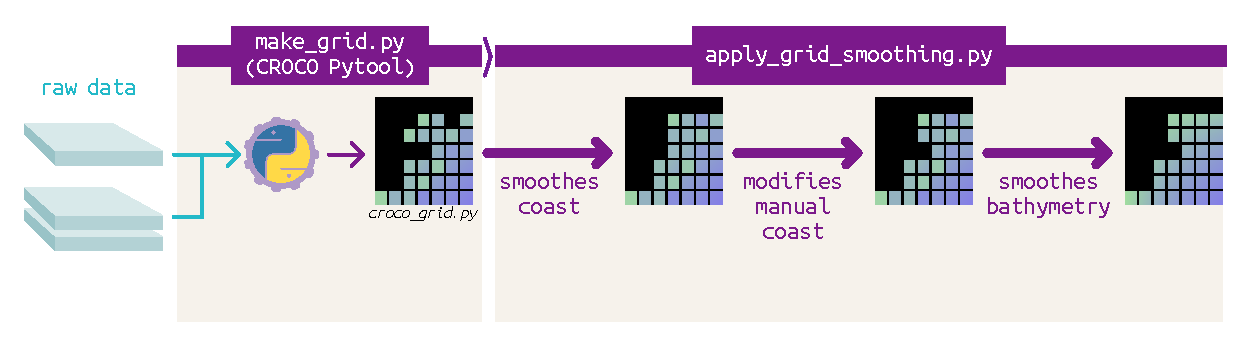
\includegraphics[scale=0.7]{../images/workflow/grid_smoothing.pdf}
    \caption{Organisation des étapes de traitement effectuées par le nouveau code de calcul \textit{apply\_grid\_smoothing.py} suite à l'utilisation de l'outil original \textit{make\_grid.py}.}
    \label{fig:new_smooth_work}
    
\end{figure}
\begin{figure}[h!]
    \centering
    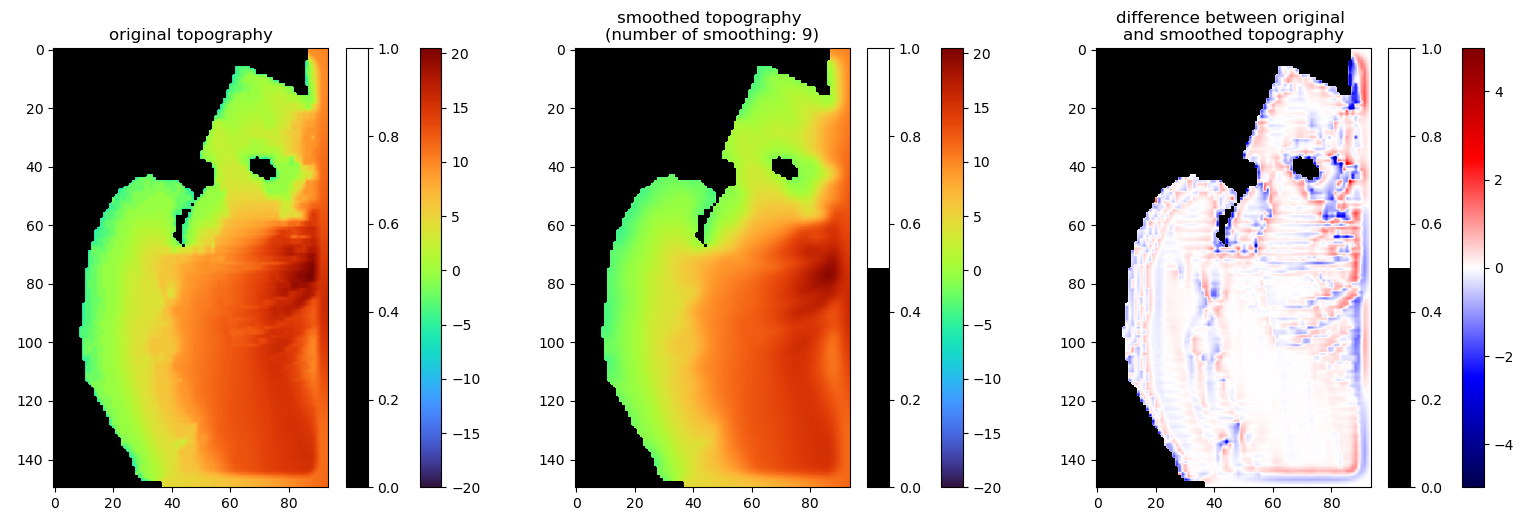
\includegraphics[scale=0.35]{../images/grid_smoothing_adcl5_9.png}
    \caption{
        \textbf{Visualisation du nouvel l'outil de traitement du domaine MACLoup.}\\
        \textbf{À gauche}, le domaine original, les teintes de couleurs correspondent à la bathymétrie par rapport au niveau marin moyen.
        Une valeur positive correspond à une hauteur en dessous du niveau marin.
        Les pixels sont noirs au niveau du masque qui identifie les zones émergées.
        Un pixel représente une surface de $75$ par $75~m$.
        \textbf{Au centre}, le domaine modifié.
        La bathymétrie est lissée et le masque est complété
        \textbf{À droite}, carte des différences de bathymétrie entre le domaine original et modifié.
        Cette carte permet notamment de vérifier que les valeurs n'ont pas été modifiées aux limites externes du domaine.
    }
    \label{fig:new_smooth}
\end{figure}

La Figure \ref{fig:workflow_prepro_main} présente l'utilisation des CROCO Pytools modifiés et des scripts écrits dans le cadre du stage pour l'ensemble des opérations de pré-traitement.
Les chemins de fichiers présentées dans le rapport correspondent à la nomenclature définie en Annexes \ref{anx:orga_fichiers}.

\begin{figure}[h!]
    \begin{center}
        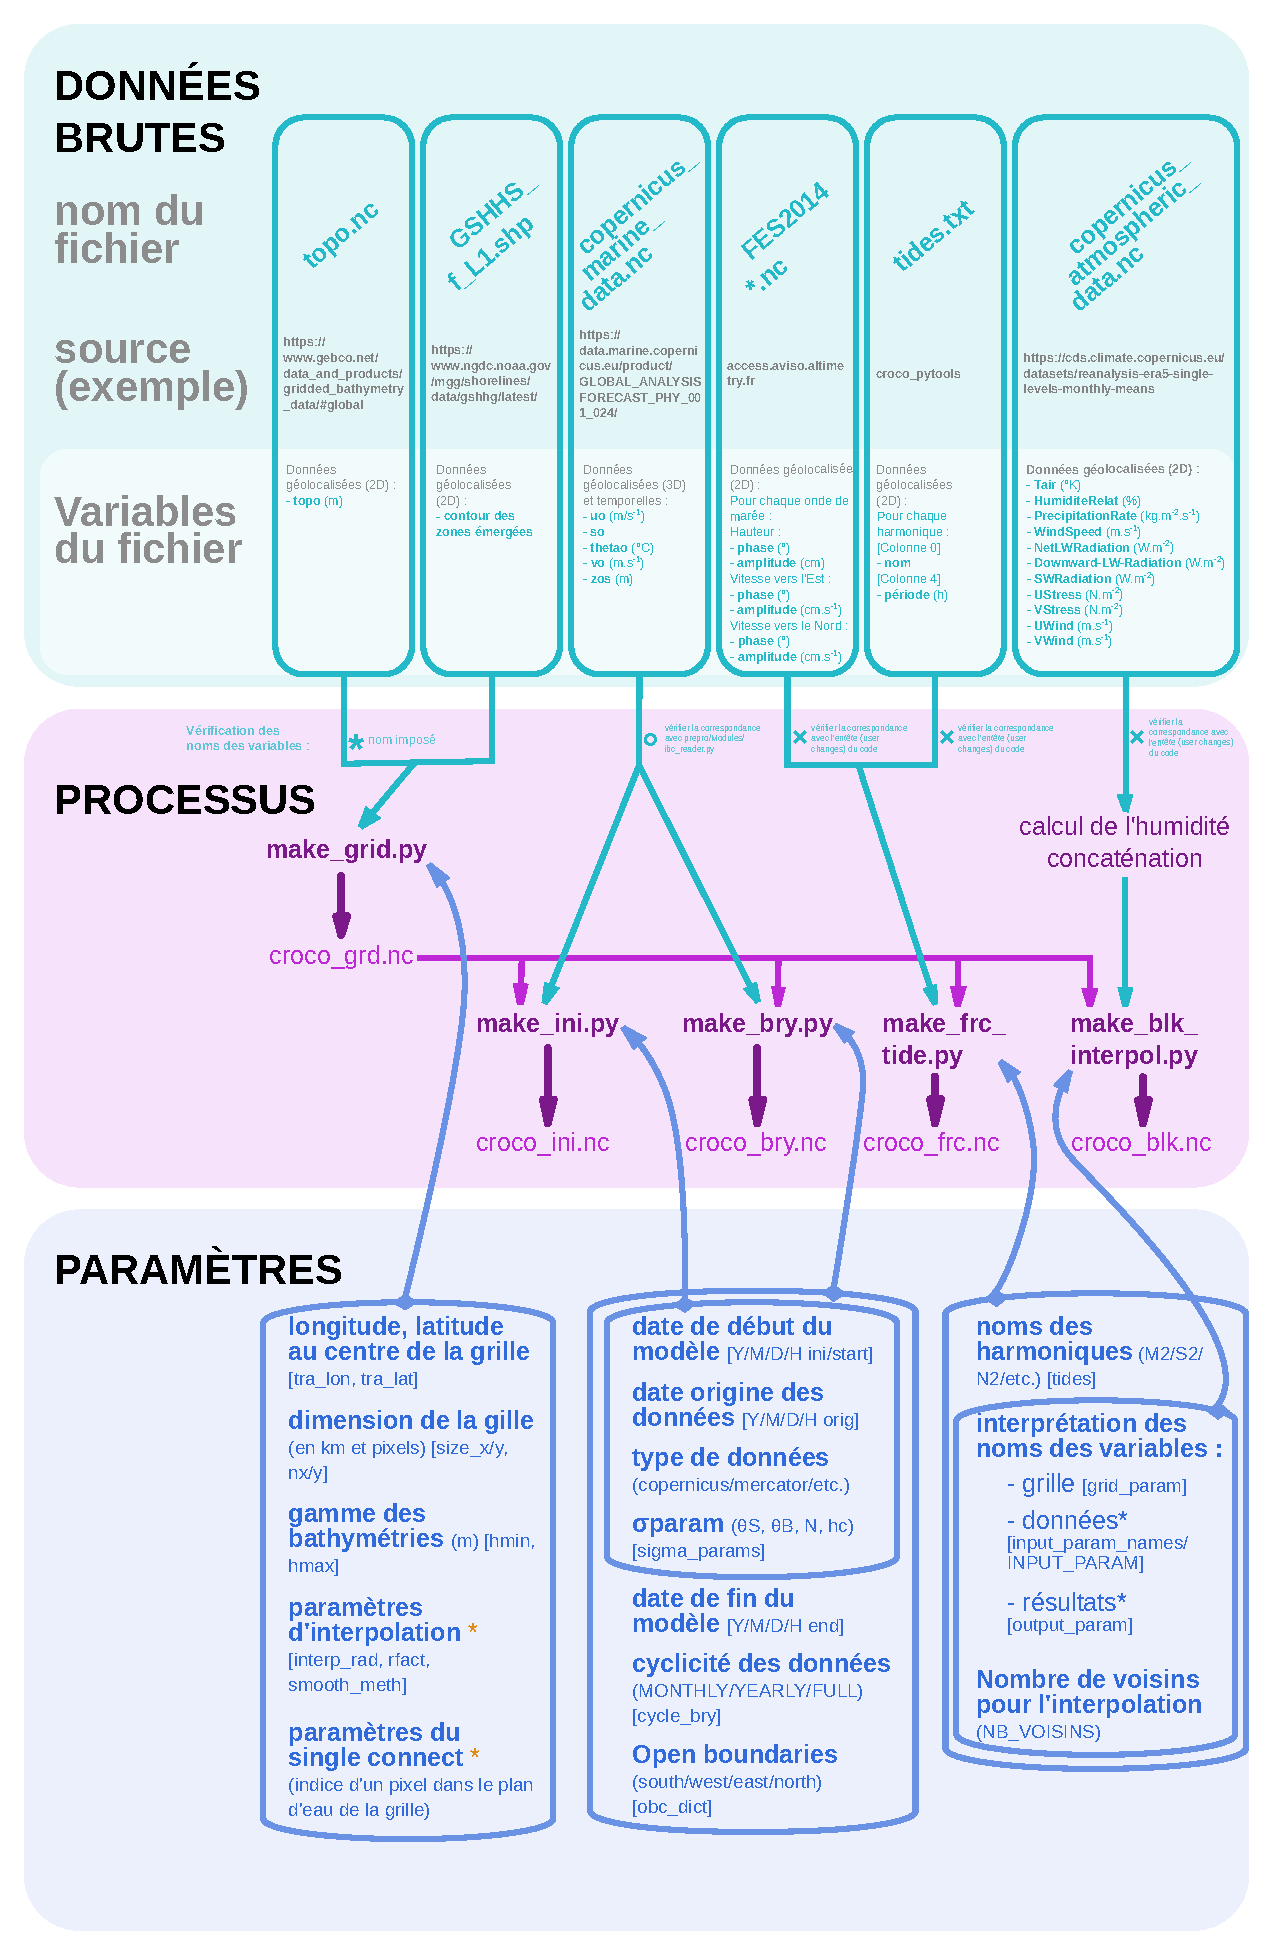
\includegraphics[scale=0.35]{../images/workflow/graphe_data_process_mere.pdf}
        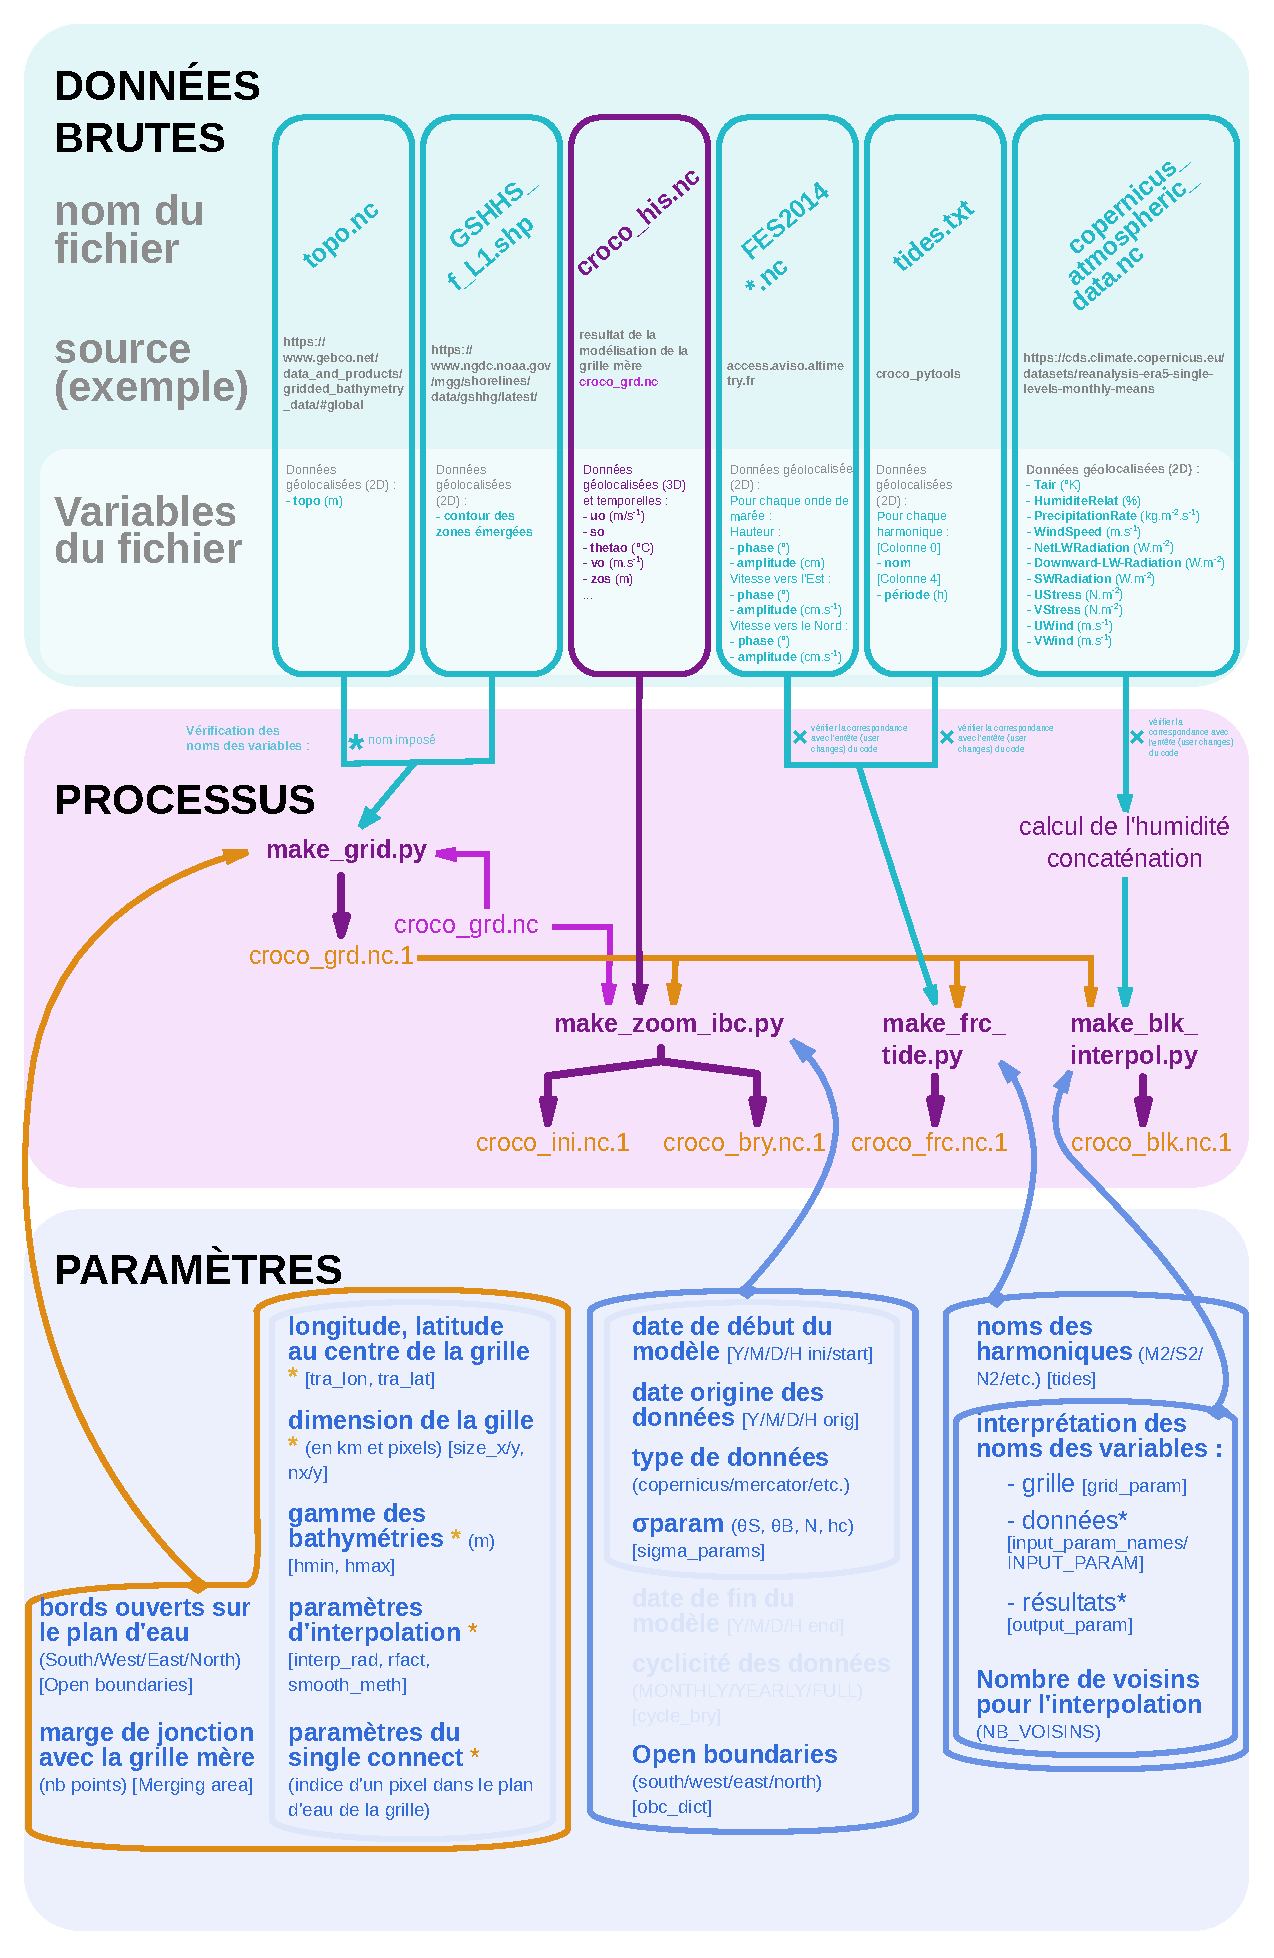
\includegraphics[scale=0.35]{../images/workflow/graphe_data_process_fille_zoom.pdf}
        \caption{
            [à simplifier sur la partie "données brutes"]
            \textbf{Pré-traitement avec les CROCO Pytools pour une grille simple ({\color{workColor}mère}) à gauche et pour une sous-grille imbriquée ({\color{orange}fille}) à droite.}
            \\Les paramètres marqués d'une {\color{paramColor}astérisque (*) bleue} sont ceux qui doivent être modifiés en fonction du code pour lesquels ils sont utilisés (\textit{make\_frc\_tide.py} ou \textit{make\_blk\_interpol.py}).
            Les paramètres marqués d'une {\color{orange}astérisque (*) orange} sont des paramètres qui ont la même signification pour la grille mère et pour la grille fille mais leur valeur peut être différente pour chaque grille.
            Dans les données brutes de la grille fille, {\color{outputColor}croco\_his.nc} provient de l'exécution du modèle CROCO sur la grille mère {\color{workColor}croco\_grd.nc}.
            La signification des paramètres cités dans la figure est détaillée en Annexes.
        }
        \label{fig:workflow_prepro_main}
    \end{center}
\end{figure}




%Les deux fichiers de forçage restants - les forçages par la marée et atmosphériques \ref{par:forcages_atm} - ont été générés à partir de données brutes par deux scripts Python développés dans le cadre du stage.
%En effet, les CROCO Pytools associés à ces forçages n'étaient pas existants ou pas fonctionnels avec nos données.


\textbf{Les forçages par la marée}\\
%\label{par:forcages_marree}
%Le script \textit{make\_frc.py}, écrit dans le cadre du stage, permet de générer un fichier de marée pour CROCO à partir des données des modèles TPXO10 ou FES2014.
%Les données procurées par les modèles de marées sont les amplitudes et les phases des hauteur d'eau et des composantes des courants associées à différentes harmoniques de marées en fonction de la position à la surface du globe.
%Les données que doit contenir le fichier \textit{make\_frc.py} sont les amplitudes et phases des hauteur d'eau et les paramètres de l'ellipse représentative des courants de marée.
%Une conversion doit donc être effectuée dans le script \textit{make\_frc.py}.
%La conversion utilise les formules utilisée dans la fonction ap2ep dans le code des CROCO Pytool de référence.
%Cette fonction est définie par \cite[Zhigang Xu (2002)][]{ap2ep} dans une fonction matlab similaire à celle des CROCO Pytools.
%Les équations résumant les opérations effectuées par la fonction ap2ep sont détaillées en Annexe (\ref{anx:ap2ep}).
%Les données de marée du modèle TPXO10 ont été testées, mais ce sont les résultats du modèle FES2014 qui ont finalement été retenus notamment car ils contiennent un nombre plus important d'harmoniques de marées.
%Si les données de FES2022 sont complétées dans le futur, il sera alors possible d'aisément re-modéliser les domaines avec les nouvelles données.
%(indiquer pourquoi ? meilleure résolution dans notre zone, données à un format plus adapté au pré-processing)

\textbf{les forçages atmosphériques}\\
\label{par:forcages_atm}
Le script \textit{make\_blk.py}, écrit dans le cadre du stage, génère un fichier de conditions atmosphériques en surface de l'eau à partir des données issues de Copernicus (climate).
Ces données sont toutes celles attendues dans le fichier de conditions atmosphériques à l'exception de l'humidité relative au dessus de la surface de l'eau. Cette dernière donnée n'est pas disponible dans le pool de données utilisées.
Toutefois, la température du point de rosée de l'eau est disponibles dans ce pool.
Or, la température du point de rosée est dépendante de plusieurs paramètres atmosphériques dont l'humidité relative.
Une conversion permettant d'estimer l'humidité relative a donc été ajouté dans le script \textit{make\_blk.py}.
Le calcul des valeurs d'humidité relative $RH$ suit le méthode décrite par \cite{humidity_formulation} en considérant une température entre $-20$ et $+50 ^\circ C$ :
$$RH = 10^{7,591386.(\frac{T_{dewpt}}{T_{dewpt}+240,7263}-\frac{T}{T+240,7263})}$$
avec $T_{dewpt}$ la température du point de rosée de l'air à $2~m$ au dessus de la surface de l'eau et $T$ la température de l'air à la même altitude.

\subsubsection{Données brutes utilisées}

L'ensemble des données brutes utilisées pour la génération des données d'entrées est représenté en Figure \ref{fig:workflow_prepro_main}.

Pour la majorité de la surface couverte par la grille mère, les données de bathymétrie proviennent de GEBCO 2024.
Ces données couvrent l'espace selon une grille régulière.
Par ailleurs, deux campagnes offrent des données de haute résolution mais discontinues sur la zone de l'anse du Cul-de-Loup.
La campagne du ROL (https://www.rolnhdf.fr/) constituée de deux phases (topo-bathymétrique de 2016 à 2018 et topographique et orthophoto en 2020) couvre les côtes Normandes.
Les données de cette campagnes utilisées pour l'étude de l'anse du Cul-de-Loup proviennent de prises Lidar.
La campagne XXX a été réalisée dans le but de compléter les données de la campagne ROL.
Les données provenant de GEBCO, ROL et XXX sont donc fusionnées entre elles afin d'obtenir une cartographie bathymétrique uniforme de haute résolution dans les zones où les données le permettent.
\\
Enfin, les fichier vectoriels géo-référencés qui définissent le trait de côte proviennent de la National Oceanic and Atmospheric Administration (NOAA).


\textbf{Les conditions initiales}\\
\label{par:cond_init}
%Le fichier "croco\_ini.nc" est généré avec le script \textit{make\_ini.py} pour le domaine parent.
Les données utilisées sont alors celles des bases de données de Copernicus (marine).
Ces données sont : la température et la salinité %, les conditions atmosphériques, (vérifier si plus de données).


\textbf{Les conditions aux bordures}\\
\label{par:cond_bords}
%Le fichier "croco\_bry.nc" est généré avec le script \textit{make\_bry.py} pour le domaine parent.
Les données utilisées sont alors celles des bases de données de Copernicus (marine).
Ces données sont : la température et la salinité %, les conditions atmosphériques, (vérifier si plus de données).


\subsection{Post-traitement}
\label{sub:postpro}
Un post-traitement des données produites par le modèle MACLoup est nécessaire pour permettre leur validation et leeur interprétation.
Ces opérations qui permettent d'extraire et de transformer certaines parties du jeu de données.
La fast fourrier transform (FFT, \alert{citation*}) a été utilisée, c'est l'une des méthodes classiques d'analyse fréquentielle des données.
Pour la comparaison entre les données réelles (données PROTEC) et les données modélisées avec MACLoup, c'est la maille la plus proche de la localisation réelle de l'enregistrement PROTEC qui est utilisée pour effectuer des comparaisons.

%à voir, détailler :
%\begin{itemize}
%    \item l'écriture de scripts pour extraire le point le plus proches,
%    \item les choix pour les interpolations (closest neighbor),
%    \item les REQM utilisés (RMSEDEI).
%\end{itemize}


\newpage
\section{RÉSULTATS}
\label{sec:resultats}

%{\color{lightgrey}
    %Mettre les résultats uniquement.
    %}

\subsection{Le modèle "anse du Cul-de-Loup"}
\label{sub:modele_ADCL}

%[propriété des grilles en premier (+ important)]

%[acronyme pour modèle ?]

%{\color{lightgrey}
    %    Grosse partie dans laquelle il va falloir expliquer les différentes étapes de mis en place du modèle ADCL (pour la mise en place non spécifique à la zone, partie précédente ?) détailler les paramètres choisis.
    %}

La lecture de la documentation, des codes des CROCO Pytools et de fichiers d'exemple de sortie du pré-traitement Matlab ont permis de réaliser des choix pour le pré-traitement.
Ce dernier à aboutit à la préparation correcte des fichiers pour l'exécution du code CROCO.
Les choix qui ont été faits sont détaillés dans les parties suivantes.


\subsubsection{Paramètres généraux choisis}
\label{subsub:param_generaux}
%{\color{lightgrey}
%    Paramètres de la grille (étendue, localisation, résolution horizontale et verticale, etc.), choix du LES.
%}

Les paramètres généraux sont majoritairement déterminés par l'utilisateur·ice lors de l'exécution du CROCO Pytool de création de la grille.
Cette grille est fondamentale au fonctionnement de CROCO, elle détermine en quels point sont résolues les équations du modèle. Ses principales propriétés sont :

\begin{itemize}
    \item sur chaque plan horizontal, la grille couvre la même zone rectangulaire sur Terre, à l'exception des zones émergées,
    \item les espacement en latitude et longitude des mailles sont réguliers.
\end{itemize}

D'autre part, les propriétés verticales ($\sigma_{param}$) de la modélisation sont d'une grande importance, notamment pour la qualité de la résolution des turbulences et des mélanges avec la surface du plan d'eau.
Ces propriétés ne sont pas directement déterminées dans le fichier contenant la grille CROCO.
Toutefois, les $\sigma_{param}$ doivent être fixés par l'utilisateur·ice dans les différents CROCO Pytools de génération des conditions initiales et aux limites, comme représenté dans la Figure \ref{fig:workflow_prepro_main}.

\begin{itemize}
    \item le nombre de points alignés verticalement est constant quelque soit la bathymétrie dans le plan d'eau,
    \item les espacements verticaux entre les mailles de la grille sont variables. Ils respectent les paramètre $\theta_s$, $\theta_b$, $hc$ et $n$ qui imposent des répartitions verticales respectant la bathymétrie en chaque point comme illustré par la Figure \ref{fig:vertical_resolution}.
\end{itemize}


Les paramètres entrés par l'utilisateur·ice fixent la localisation en latitude et longitude de la grille, sa résolution dans les trois dimensions de l'espace ainsi que le choix de la restriction de la modélisation à un seul plan d'eau.
De plus, la grille est générée en utilisant les données brutes de bathymétrie et de trait de côte, comme décrites dans la partie précédente.

La localisation et l'étendue spatiale de la grille sont choisies afin que ses faces ouvertes sur le plan d'eau soient le moins possible recoupées par des zones émergées.


\subsubsection{propriétés des grilles}
\label{subsub:propriete_gilles_ADCL}
%{\color{lightgrey}
    %    Nombre et paramètres des grilles imbriquées
    %}

La zone d'étude a un rayon d'une dizaine de kilomètre et la résolution des données attendues est d'au moins quelques dizaines de mètre.
Toutefois, les données brutes (les modèles de marées et les données générales marines et atmosphérique) qui sont utilisées pour fixer les conditions initiales et aux limites pour un modèle dans cette zone ont une résolution largement inférieure à celle attendue en sortie de modèle.
Il est donc intéressant de mettre en place un ensemble de modélisations en grilles emboîtées afin de décrire correctement les courants autour du Nord du Cotentin.
L'imbrication successive des grilles permet d'aboutir à la modélisation plus réaliste et stable numériquement d'une zone restreinte à l'anse du Cul-de-Loup.
Trois grilles emboîtées ont ainsi été réalisées ici, elles sont illustrées en Figure \ref{fig:imbrication}.


La position des grilles emboîtées est déterminée selon deux règles :
\begin{itemize}
    \item les bords de la grille fille doivent être assez loin des bords ouverts sur le plan d'eau de la grille mère, leur centre est donc généralement proche,
    \item au niveau de l'intersection entre les bords d'une grille et le tracé de la côte, ce dernier doit être le plus simple possible, c'est à dire de préférence rectiligne en Nord-Sud ou Est-Ouest.
    De plus, pour les grilles filles, le tracé de la côte au niveau des bords doit être aligné avec le tracé de la côte de la grille mère.
\end{itemize}

Les paramètres principaux des deux domaines emboîtés sont décrits en Table\ref{table:param_generaux}.

\begin{table}[h!]
    \centering
    
    \begin{tabular}{||c||c|c|c|c|c|}
        \hline
        Nom du domaine & latitude & longitude & étendue Nord Sud & étendue Est Ouest & résolution (m/px)\\
        & au centre & au centre &  &  & \\
        \hline
        Cotentin & 49,6 & -1,28 & $80~pixels$, $150~km$ & $80~pixels$, $150~km$ & $1~875$\\
        ADCL & 49,566 & -1,27 & $220~pixels$, $11~km$ & $138~pixels$, $6,9~km$ & $50$\\
        \hline
    \end{tabular}\newline
    
    \begin{tabular}{||c||c|c|c|c|c|c|}
        \hline
        Nom du domaine & nombre de & lissage de & source de & marge de jonction & $\sigma_{s}$ & $\sigma_{b}$ \\
        & couches $\sigma$ & la bathymétrie & bathymétrie & de la bathymétrie &  & \\
        \hline
        Cotentin & 30 & 0 & GEBCO & - & 0  & 2 \\
        ADCL & 5 & 9 & ROL et XXX & $5~pixels$ & 0 & 2 \\
        \hline
    \end{tabular}\newline
    
    \begin{tabular}{||c||c|c|c|}
        \hline
        Nom du domaine & bords ouverts & source des forçages & source des forçages \\
        &  & de marée & initiaux et aux limites \\
        \hline
        Cotentin & Nord Sud Est Ouest & FES 2014 & Copernicus \\
        ADCL & Nord Sud Est & - & COTENTIN \\
        \hline
    \end{tabular}
    \caption{
        Paramètres généraux des domaines de MACLoup mis en place pour obtenir les résultats du rapport.
        Les domaines auxiliaires explorés durant le stage et les raisons de leur non-utilisation sont présentés en Annexes (\ref{anx:param_generaux_aux})\alert{/ ne sont pas présentés ici.}.
    }
    \label{table:param_generaux}
\end{table}

\subsection{Sortie de modèle}
\label{sub:sortie_modele}
De nombreuses données peuvent être extraites de la modélisation, afin de limiter le poids des fichiers obtenus, seules certaines variables ont été sélectionnées pour l'enregistrement.
On s'intéressera ici aux

%Sorties selon les choix de modélisation:
%\begin{itemize}
%    \item mode hydro (RANS, LES, etc.) (à voir)
%    \item effet de l'atmosphère (bulk / climato)
%    \item couplage avec les vagues (WaveWatch-III) (pas encore fait)
%\end{itemize}

Visualisation : snapshots représentatifs de la marée, zoom sur des zones dynamiques

Comparaisons : différences, variations de l'écart type

\subsubsection{Résultats bruts}
Phrase intro : comment représenter le modèle ?

patchwork 6h pour voir la marée

var T et S (sur deux extrêmes de courants)

graphe var vitesse et etc. en un point selon le temps.

mise en évidence des gyres, du fonctionnement du wet-dry

\subsubsection{Analyses des choix de modélisation}
Comparaison des sorties avec plus ou moins d'harmoniques de marée

Effet de l'ajout d'une topo plus précise

Effet de l'ajout du bottom drag (à voir)

\newpage

\section{DISCUSSION}
\label{sec:discussion}



\subsection{Données de validation - Le projet PROTEC}
\label{subsub:protec}

Le "Projet de Territoire : anse du Cul-de-Loup" (PROTEC) s'est déroulé de juin 2022 à juin 2024. Financé par l'Agence de l'Eau Seine-Normandie (AESN), ce programme de recherche était sous la responsabilité de G. Gregoire (MCF au Cnam/Intechmer) et a intéressé plusieurs autres membres de l'équipe du Cnam/Intechmer. L'objectif de PROTEC a été de dresser un état des lieux environnementale de l'anse du Cul-du-Loup, principalement sur les aspects en relations avec les sédiments, leur dynamique actuelle et passée (Fig. \ref{fig:sed-adcl}).

\begin{figure}[!h]
    \centering
    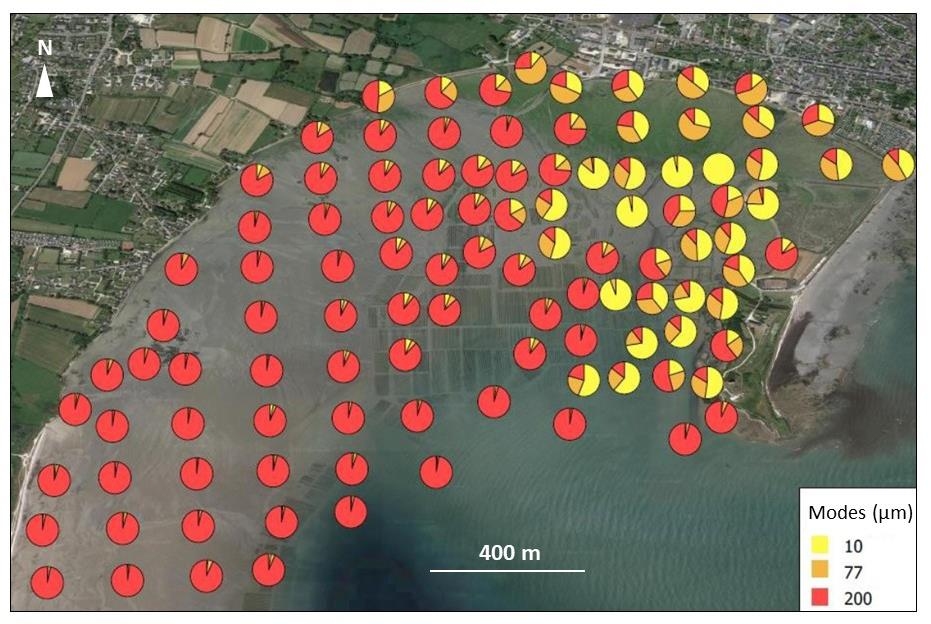
\includegraphics[width=0.8\linewidth]{../images/sed_adcl_protec.png}
    \caption[Sédiment de l'anse du Cul-de-Loup]{Pourcentages relatif des principales fractions granulométriques dans des échantillons sédimentaires de surface prélevés dans l'anse du Cul-de-Loup (jaune - 10 $\mu$m, orange - 77 $\mu$m, rouge - 200 $\mu$m).}
    \label{fig:sed-adcl}
\end{figure}

%\subsection{Données externes utilisées}
%\label{sub:donnees_externes}
%Les données obtenues durant la campagne PROTEC sont utilisées pour analyser la justesse des résultats de la modélisation.
%Ces données couvrent la période de novembre 2023 à mai 2024.

%[description de l'obtention des données]


Comparaison des résultats du modèle avec les mesures de terrain: graphiques

\subsubsection{Erreur quadratique moyenne}
indicateurs de qualité (RMSE, etc.)

\subsubsection{Analyse fréquentielle}
(marée = principal critère validation modèles)
Comparaison en analyse fréquentielle (sur l'ensemble de l'enregistrement)

Analyse en fréquence par rapport aux données de FES et en relatif selon la localisation sur la grille

\newpage

\section{CONCLUSION}
\label{sec:conclusion}

Ca sera fait à la fin ou presque
bilan + perspective

\newpage
\section{BIBLIOGRAPHIE}
%\bibliography{../rapport-AB.bib}
%\bibliography{../bibliography.bib}
\printbibliography

\newpage
\section{ANNEXES}
\label{annexes}
\subsection{Répartition des variables dans les mailles}
Les variables que nous avons choisies de modéliser sont organisées comme suit entre les localisations sur les mailles de \cite{Arakawa_C-grid_1977}.\\
La majorité des variables sont localisées en \textbf{position H}, sur le maillage central.
\begin{itemize}
    \item la hauteur de la colonne d'eau relativement au niveau marin moyen (*référentiel à vérifier),
    \item la température de l'eau,
    \item la salinité de d'eau,
    \item l'ensemble des paramètres décrivant les ondes de marée (phase et amplitude de la hauteur d'eau ainsi que celles des deux composantes des courants induits),
    \item l'ensemble des paramètres atmosphériques à l'exception du vent (précipitation, température de l'air, vitesse absolue et direction du vent à $10~m$ au dessus de la surface de l'eau, etc.).
\end{itemize}
Les paramètres localisés à la \textbf{position U}, sur un second maillage :
\begin{itemize}
    \item la composante Est-Ouest de la vitesse de déplacement de l'eau,
    \item la contrainte à la surface de l'eau causée par la composante Est-Ouest du vent,
    \item la composante Est-Ouest de la vitesse de déplacement de l'air à $10~m$.
\end{itemize}
Enfin, les paramètres localisés à la \textbf{position V}, sur un troisième:
\begin{itemize}
    \item la composante Nord-Sud de la vitesse de déplacement de l'eau,
    \item la contrainte à la surface de l'eau causée par la composante Nord-Sud du vent,
    \item la composante Nord-Sud de la vitesse de déplacement de l'air à $10~m$.
\end{itemize}

%L'ensemble de ces paramètres ne sont ni exprimés ni pris en compte aux points indiqués comme émergés par la grille.
Indépendamment de leur appartenance à l'un ou l'autre des maillages, les paramètres forçant le modèle ne couvrent pas toujours l'ensemble du maillage.
Certains de ces paramètres sont exprimés sur l'intégralité du maillage horizontal et vertical.
D'autres ne le sont qu'aux bords du maillage, parfois sur l'ensemble des mailles verticales.
D'autres encore sont exprimés sur toutes l'étendue horizontale de la grille mais sur une unique maille à la verticale, ces données sont localisées soit en surface (ex. vent) soit au fond (ex. rugosité).

\subsection{Méthode d'emboîtement AGRIF}
\label{anx:AGRIF}
AGRIF est un type d'emboîtement de domaines est une méthode adaptative de raffinement de grilles en Fortran (AGRIF\footnote{AGRIF : Adaptive Grid Refinement In Fortran}).
L'emboîtement des domaines est simultané et rétrospectif
Ce qui signifie que tous les domaines sont générées avec les données du pré-traitement avant la modélisation.
Ensuite, pendant la modélisation, sont utilisées alternativement les données du-des modèles parents pour les conditions aux bords du-des domaines enfants puis les valeurs au bords du-des domaines enfants pour contraindre celles au sein du-des domaines parents.
Ce système d'emboîtement simplifie le processus de modélisation pour l'utilisateur·ice qui n'a besoin de mettre en place et de démarrer le modèle qu'une unique fois pour obtenir les résultats de haute résolution des domaines enfants.
D'autre part, il a plus de chances de mieux représenter la réalité grâce à son fonctionnement en aller retour entre les grilles,

\subsection{Domaines auxiliaires}

\begin{table}[h!]
    \centering
    (à faire)
    \begin{tabular}{||c||c|c|c|c|c|}
        \hline
        Nom du domaine & latitude & longitude & étendue Nord Sud & étendue Est Ouest & résolution (m/px)\\
        & au centre & au centre &  &  & \\
        \hline
        Cotentin & 49,6 & -1,28 & $80~pixels$, $150~km$ & $80~pixels$, $150~km$ & $1~875$\\
        MACLoup\_4 & 49,566 & -1,27 & $220~pixels$, $11~km$ & $138~pixels$, $6,9~km$ & $50$\\
        \hline
    \end{tabular}\newline
    
    \begin{tabular}{||c||c|c|c|c|c|c|}
        \hline
        Nom du domaine & nombre de & lissage de & source de & marge de jonction & $\sigma_{s}$ & $\sigma_{b}$ \\
        & couches $\sigma$ & la bathymétrie & bathymétrie & de la bathymétrie &  & \\
        \hline
        Cotentin & 30 & 0 & GEBCO & - & 0  & 2 \\
        MACLoup\_4 & 5 & 9 & ROL et XXX & $5~pixels$ & 0 & 2 \\
        \hline
    \end{tabular}\newline
    
    \begin{tabular}{||c||c|c|c|}
        \hline
        Nom du domaine & bords ouverts & source des forçages & source des forçages \\
        &  & de marée & initiaux et aux limites \\
        \hline
        Cotentin & Nord Sud Est Ouest & FES 2014 & Copernicus \\
        MACLoup\_4 & Nord Sud Est & - & COTENTIN \\
        \hline
    \end{tabular}
    \caption{
        Paramètres généraux des domaines auxiliaires explorés durant le stage et les raisons de leur non-utilisation.
    }
    \label{anx:param_generaux_aux}
\end{table}


\subsection{Schémas numériques}
\subsubsection{Schéma WENO de cinquième ordre (Weighted Essentially Non-Oscillatory scheme)}\label{anx:WENO}
Les variables sont disposées en C-grille d'Arakawa.
Les valeurs des traceurs sont notées $q_i$ et les vitesses $u_i$.
Dans le cadre de ce schémas d'advection, trois valeurs aux interfaces sont évaluées en se utilisant trois stencils différents. Une moyenne non linéaire entre ces trois valeurs est utilisée comme suit pour déterminer la valeur calculée :
$$\tilde{q}_{k-\frac{1}{2}} = a_1k-\frac{1}{2}^{(1)} + a_2k-\frac{1}{2}^{(2)} + a_2k-\frac{1}{2}^{(2)}$$
Les constantes de pondération sont définies selon les règles suivantes :
\begin{enumerate}
    \item $\sum_{j=0}^{2}a_j = 1$,
    \item propriété ENO (Essentially Non Oscillatory),
    \item cinquième ordre à condition que q(x) soit peut rugueux.
\end{enumerate}
C'est un schéma à variation bornée (TBV, Total variation Bounded).
source pour l'équation et son explication : \cite{schemas_advection}


\subsection{Fichiers d'entrées}
\subsubsection{cppdefs.h}
\label{anx:cppdefs}
Le contenu du fichier \textit{cppdefs.h} des grilles filles est écrit ci-dessous. Pour la grille mère, comme il n'y a pas de données héritées d'une grille précédente, quelques clefs sont modifiées selon la table \ref{table:cppdefs_mere}.

\begin{table}[h!]
    \centering
    \begin{tabular}{c | c c c}
        BSTRESS\_FAST & define & $\rightarrow$ & {\color{red}undef}\\
        \hline
        LIMIT\_BSTRESS & undef & $\rightarrow$ & {\color{green}define}\\
        \hline
        SPONGE & undef & $\rightarrow$ & {\color{green}define}\\
        \hline
        TIDE & undef & $\rightarrow$ & {\color{green}define}\\
    \end{tabular}
    \caption{
        Modifications à appliquer au fichier cppdefs d'une grille fille dont un exemple est donnée dans l'encadré en section \ref{codecppdefs} pour obtenir celui de la grille mère.
        Le statut de la clefs dans le fichier de la grille fille est écrit en colonne centrale, le statut dans le fichier de la grille mère est indiqué en colonne de droite.
    }
    \label{table:cppdefs_mere}
\end{table}

% peut être à transformer en un tableau pour une meilleure lisibilité
% + nettoyer
\begin{codeEnv}{{Contenu du fichier cppdefs.h d'une sous-grille\label{codecppdefs}}}
    \lstinputlisting[firstline=3,lastline=386,language=bash]{../croco_files/cppdefs_child.h}
\end{codeEnv}

\subsection{Nomenclature et organisation des fichiers de la configuration}
\color{darkgrey}
\label{anx:orga_fichiers}
\dirtree{%
    .0 ~/\DTcomment{le chemin peut être différent pour PATH-TO-CROCO/ et PATH-TO-CONFIG/}.
    .1 PATH-TO-CROCO/.
    .2 croco/\DTcomment{dossier généré par l'installation de croco}.
    .3 OCEAN/.
    .3 SCRIPTS/.
    .3 MUSTANG/.
    .3 AGRIF/.
    .3 create\_config.bash.
    .3 version.txt.
    .3 REANDME.md.
    .3 CHANGELOG.md.
    %
    .2 croco\_pytools/\DTcomment{dossier généré par l'installation des outils python (CROCO Pytools)}.
    .3 prepro/.
    .4 Modules/.
    .5 tides.txt.
    .4 Readers/.
    .5 ibc\_reader.py.
    .5 topo\_reader.py.
    .4 make\_grid.py.
    .4 make\_ini.py.
    .4 make\_bry.py.
    .3 make\_blk\_interpol.py.
    .3 make\_frc\_tide.py.
    %
    .1 PATH-TO-CONFIGS/.
    .2 CONFIGS/\DTcomment{dossier pouvant être généré avec create\_config.bash (modifié selon la partie \ref{create_config})}.
    .3 CONFIG-NAME/.
    .4 datasets/.
    .5 Bry/.
    .6 AVISO/.
    .7 FES2014*.nc.
    .6 ../Ini/copernicus\_marine\_data.nc.link.
    .5 Bulk/.
    .6 cpernicus\_atmospheric\_data.nc.
    .5 gshhs/.
    .6 GSHHS\_f\_L1.shp.
    .5 Ini/.
    .6 copernicus\_marine\_data.nc.
    .5 Topo/.
    .6 topo.nc.
    .4 CROCO\_FILES/\DTcomment{données d'entrée pour le modèle provenant du pré-processing}.
    .4 OUTPUTS/\DTcomment{dossier d'écriture des sorties du modèle}.
    .5 croco\_his.nc.
    .5 croco\_avg.nc.
    .5 croco\_rst.nc.
    .4 cppdefs.h.
    .4 param.h.
    .4 jobcomp.
    .4 croco.in.
}
\color{black}

\subsection{Fonction ap2ep (Zhigang Xu (2002))}
\label{anx:ap2ep}
La fonction ap2ep décrite par \cite[Zhigang Xu (2002)][]{ap2ep} permet de transformer les amplitudes ($AmpleU$ et $AmplV$) et phases ($PhaseU$ et $PhaseV$) des courants de marée en paramètres d'ellipse représentant ces mêmes courants: le demi grand-axe $SemiMajAxis$, l'excentricité $Eccentricity$, l'inclinaison $Inclinaison$ et l'angle de phase $PhaseAngle$.
Les opérations effectuées respectent ces équations :
$$SemiMajAxis = \abs{wp}+\abs{wm}$$
$$Eccentricity = \frac{\abs{wp}+\abs{wm}}{\abs{wp}-\abs{wm}}$$
$$Inclinaison = \frac{arg(wm)+arg(wp)}{2\pi}.180$$
$$PhaseAngle =  \frac{arg(wm)-arg(wp)}{2\pi}.180$$
avec
\begin{equation*}
    wp = \frac{u*+j.v*}{2}
    \quad\mathrm{et}\quad
    \overline{wm} = \frac{u*-j.v*}{2}
\end{equation*}
avec
\begin{equation*}u* = \exp\left(\frac{\pi PhaseU}{180}.(-1j)\right).AmplU
    \quad\mathrm{et}\quad
    v* = \exp\left(\frac{\pi PhaseV}{180}.(-1j)\right).AmplV
\end{equation*}
avec $PhaseU$, $PhaseV$, $AmpleU$, $AmplV$ les phases et amplitudes des composantes respectivement Sud-Ouest et Nord-Sud de la vitesse d'une onde de marée.

\newpage
\section{ANNEXES À ORGANISER / RETIRER (ancien Matériel et Méthode)}

\subsection{Le code de calcul CROCO}

mettre les principes généraux de CROCO (origine, type de modèle, etc...)

+ organisation des fichiers



\subsubsection{Processus généraux}

\textbf{Installation}

Explication de l'installation des CROCO Pytools, de croco et de l'activation de l'environnement Anaconda/Miniconda \textit{croco\_pyenv}.

\begin{codeEnv}{installation de croco}
    \begin{lstlisting}[language=bash]
        # en se placant dans PATH-TO-CROCO/
        git clone --branch v2.0.1 https://gitlab.inria.fr/croco-ocean/croco.git croco-v2.0.1
    \end{lstlisting}
\end{codeEnv}

\begin{codeEnv}{installation de miniConda}
    \begin{lstlisting}[language=bash]
        wget https://repo.anaconda.com/miniconda/Miniconda3-latest-Linux-x86_64.sh
        sudo chmod +x Miniconda3-latest-Linux-x86_64.sh
        bash Miniconda3-latest-Linux-x86_64.sh -p $HOME/miniconda3
        source $HOME/miniconda3/bin/activate
        conda init
    \end{lstlisting}
\end{codeEnv}

\begin{codeEnv}{installation des CROCO Pytools}
    \begin{lstlisting}[language=bash]
        # en se placant dans PATH-TO-CROCO/
        git clone --branch release https://gitlab.inria.fr/croco-ocean/croco_pytools.git
        cd croco_pytools/prepro/
        # conda activate croco\_pyenv
        python3 install.py
        > Do you want to install conda environment? [y,[n]]: y
        > Do you want to compile fortran tools? y,[n]: y
    \end{lstlisting}
\end{codeEnv}

Une fois croco et les CROCO Pytools installés, l'achitecture de la configuration doit être générée. Nativement, croco contient un fichier \textit{create\_config.bash} qui effetue ce travail. Toutefois, comme l'architecture choisie pour ce rapport est différente de celle de référence, un nouveau fichier \textit{create\_config.bash} a été écrit, son contenu est défini ci-après.

\begin{codeEnv}{\textbf{contenu de \textit{create\_config.bash} adapté à l’architecture choisie pour ce rapport}}\label{create_config}
    \begin{lstlisting}[language=bash]
        # croco source directory
        # ---------------------
        CROCO_DIR=~/PATH-TO-CROCO/croco
        
        # Home and Work configuration directories
        # ---------------------------------------
        MY_CONFIG_HOME=~/PATH-TO-CONFIGS/CONFIGS
        
        # croco_tools directory for matlab tools
        # ---------------------
        # TOOLS_DIR=~/PATH-TO-CROCO/croco_pytools
        # For pre-processing WITH MATLAB:
        #cp ${TOOLS_DIR}/crocotools_param.m ${MY_CONFIG_HOME}/${MY_CONFIG_NAME}/
        #cp ${TOOLS_DIR}/start.m ${MY_CONFIG_HOME}/${MY_CONFIG_NAME}/
        
        # Configuration name
        # ------------------
        MY_CONFIG_NAME=CONFIG-NAME  # put the name you want
        
        # For configuration initialisaiton
        mkdir ${MY_CONFIG_HOME}/${MY_CONFIG_NAME}
        mkdir ${MY_CONFIG_HOME}/${MY_CONFIG_NAME}/datasets
        mkdir ${MY_CONFIG_HOME}/${MY_CONFIG_NAME}/datasets/Bry
        mkdir ${MY_CONFIG_HOME}/${MY_CONFIG_NAME}/datasets/Bulk
        mkdir ${MY_CONFIG_HOME}/${MY_CONFIG_NAME}/datasets/gshhs
        mkdir ${MY_CONFIG_HOME}/${MY_CONFIG_NAME}/datasets/Ini
        mkdir ${MY_CONFIG_HOME}/${MY_CONFIG_NAME}/datasets/Topo
        
        
        # For pre-processing WITH PYTHON :
        mkdir ${MY_CONFIG_HOME}/${MY_CONFIG_NAME}/preproOUTPUT
        
        # For CROCO compiling
        cp ${CROCO_DIR}/OCEAN/cppdefs.h ${MY_CONFIG_HOME}/${MY_CONFIG_NAME}/
        cp ${CROCO_DIR}/OCEAN/param.h ${MY_CONFIG_HOME}/${MY_CONFIG_NAME}/
        cp ${CROCO_DIR}/OCEAN/jobcomp ${MY_CONFIG_HOME}/${MY_CONFIG_NAME}/
        
        # For running
        cp ${CROCO_DIR}/OCEAN/croco.in ${MY_CONFIG_HOME}/${MY_CONFIG_NAME}/
        
    \end{lstlisting}
\end{codeEnv}

\textbf{Plan général des étapes}



Le schéma Figure\ref{fig:workflow_simple} résume les étapes de décision et de traitement de données et d'exécution de codes décrit ci-après.

\begin{processEnv}{\textbf{Plan des processus généraux à suivre pour mettre en place un modèle fonctionnel}}
    
    {\color{paramColor}\textbf{Paramètres du modèle}}
    
    Avant de rechercher les données qui seraient trop lourdes à télécharger à l'échelle globale, il convient de déterminer les propriétés principales de la zone d'étude et de son modèle. Ces paramètres sont :
    
    \begin{enumerate}
        \item les latitudes et longitudes du centre de la zone d'étude totale,
        \item l'étendue en kilomètres de la zone d'étude dans le sens de la latitude et de la longitude,
        \item la gamme de bathymétrie que doit couvrir le modèle (minimum et maximum),
        \item les paramètres d'interpolation qui doivent être utilisés pour les données de bathymétrie,
        \item les coordonnées d'un point de la grille se trouvant dans le plan d'eau d'intérêt si le modèle ne doit tourner que sur un plan d'eau,
        \item les dates de début et de fin de la modélisation,
        \item les valeurs associées à la répartition des mailles verticales de la grille. Leur nombre $N$ doit aussi être déterminé.
    \end{enumerate}
    
    
    {\color{dataColor}\textbf{Données en entrée}}
    
    En entrée, les données brutes nécessaires doivent toujours couvrir spatialement l'intégralité de la zone d'étude. Elles doivent être placées dans le dossier PATH-TO-CONFIGS/CONFIGS/CONFIG-NAME/datasets/.
    Elles sont :
    
    \begin{enumerate}
        \item la bathymétrie {\color{darkgrey}[topo.nc]} couvrant au moins la zone d'étude,
        \item le masque côtier {\color{darkgrey}[GSHHS\_f\_L1.shp]} comprenant au moins les côtes de la zone d'étude,
        \item les données marines {\color{darkgrey}[copernicus\_marine\_data.nc]} couvrant une zone la plus large possible autour et comprenant la zone d'étude. Ces données doivent aussi couvrir le plus finement possible la gamme temporelle mentionnée dans la section précédente,
        \item les données issues d'un modèle global ou local de marée, par exemple TPXO10 ou FES2014 {\color{darkgrey}[FES2014*.nc]} incluant des données de hauteur d'eau et de courant pour les différentes fréquences de vagues de marée (M2, S2, N2, K2, K1, O1, P1, Q1, MF, MM,...)
        \item le fichier texte présent nativement dans les CROCO Pytools {\color{darkgrey}[tides.txt]} contenant les noms et les périodes des différentes harmoniques des vagues de marée.
        \item les données atmosphériques {\color{darkgrey}[copernicus\_atmospheric\_data.nc]} couvrant une zone large autour et comprenant la zone d'étude. Ces données doivent couvrir le plus finement possible la gamme temporelle mentionnée dans la section précédente.
    \end{enumerate}
    
    Les {\color{paramColor}\textbf{paramètres}} qu'il conviendra de récupérer dans la documentation des données de forçage (initial et aux limites) sont :
    
    \begin{enumerate}
        \item les dates qui correspondent à l'origine du temps donné dans les fichiers téléchargées (généralement 1970/01/01),
        \item la nomenclature des variables devra aussi être vérifiée en fonction du contenu de \textit{croco\_pytools/prepro/Readers/ibc\_reader.py},
        \item l'orientation des limites de la grille ouvertes dans le plan d'eau,
        \item la cyclicité potentielle des données entrées.
    \end{enumerate}
    
    {\color{workColor}\textbf{Pré-processing}}
    
    Le pré-processing des données brutes n'est détaillé ici que pour les CROCO Pytools. Les outils Matlab ne sont pas abordés.
    
    \textbf{- modifications basiques des fichiers netCDF}
    
    Certaines modifications peuvent êtres préférablement réalisées avant d'utiliser les outils de pré-processing. Ces modifications peuvent être effectuées en utilisant la librairie NCO de traitement des fichiers netCDF
    
    \begin{codeEnv}{\textbf{Changer le nom d'une variables du fichier}}
        \begin{lstlisting}[language=bash]
            # renome la variable t2m en HR
            nco chname,t2m,HR
        \end{lstlisting}
    \end{codeEnv}
    
    Cette commande n'est pas obligatoire car les fichiers "ibc\_reader.py", "make\_frc\_tide.py" et "make\_blk\_interpol.py" peuvent être adaptés à la main.
    La commande reste utile si on souhaite dupliquer une variable (La marche à suivre est : dupliquer un fichier en in1.nc et in2.nc, puis renommer la variable A en A2 du fichier nc2.nc, puis concaténer les fichiers in1.nc et in2.nc. Le fichier de sortie contient alors les deux variables identiques A et A2).
    
    \begin{codeEnv}{\textbf{Rognage des données selon une dimension}}
        \begin{lstlisting}[language=bash]
            # rogne selon les indices de la dimension time et
            # selon les valeurs des dimensions longitude et latitude
            ncks -d time,240,359 -d longitude,-2.,3. -d latitude,48.,50. in.nc out.nc
        \end{lstlisting}
    \end{codeEnv}
    
    Si des des entiers (exemple : 40) sont donnés pour la gamme à restreindre d'une dimension, ces valeurs sont interprétées comme les \textbf{indices} des dimensions minimum et maximum. Si des décimaux (exemple : 40.) sont donnés, les valeurs sont interprétées comme les \textbf{valeurs }minimales et maximales des dimensions.
    
    \begin{codeEnv}{\textbf{Concaténation de plusieurs fichiers selon les dimensions communes}}
        \begin{lstlisting}[language=bash]
            # concatene tous les fichiers data_*.nc en un fichier data_tot_calc.nc
            ncrcat raw_download/data_*.nc data_tot_calc.nc
        \end{lstlisting}
    \end{codeEnv}
    
    \begin{codeEnv}{\textbf{Effectuer une opération arithmétique sur plusieurs variables du fichier}}
        \begin{lstlisting}[language=bash]
            # calcule et stocke dans RH les valeurs d'humidite relative selon
            # les valeurs des variables d2m (temperature du point de rosee)
            # et t2m (temperature)
            ncap2 -s 'RH=10^(7.591386*(d2m/(d2m+240.7263)-t2m/(t2m+240.7263)))'\
            in.nc out.nc
        \end{lstlisting}
    \end{codeEnv}
    
    \begin{codeEnv}{\textbf{Effectuer une opération arithmétique sur plusieurs variables du fichier}}
        \begin{lstlisting}[language=bash]
            # change a "new attribute str value" la valeur de l'attribut "attribute"
            # de la variable "variable" du fichier "in.nc"
            ncatted -a attribute,variable,o,c,"new attribute str value" in.nc
        \end{lstlisting}
    \end{codeEnv}
    
    \textbf{- Génération de la grille}
    
    La grille \textit{croco\_grd.nc} est la base des prochaines actions de pré-processing ainsi que du modèle. Elle contient toutes les données relatives aux coordonnées de chaque maille de la grille sur laquelle le va travailler, ainsi que les données de bathymétrie, un paramètre de Coriolis et les coordonnées curvilinéaires des mailles.
    
    \begin{codeEnv}{\textbf{générer la grille en mode graphique}}
        \begin{lstlisting}[language=bash]
            # dans PATH-TO-CROCO/croco_pytools/prepro/
            python3 make_grid.py
            > Do you want to use interactive grid maker ?
            > (e.g., for grid rotation or parameter adjustments) : y,[n] y
        \end{lstlisting}
    \end{codeEnv}
    
    Dans la fenêtre graphique, les champs doivent être modifiés pour correspondre aux paramètres voulus. Ils peuvent être aussi déterminés et choisis par tâtonnement en utilisant les boutons \textit{Compute grid} et \textit{Compute smoothing} successivement.
    
    Les valeurs utilisées pour modéliser le Cotentin (France) ainsi que les visualisation proposées sont présentées en Figure \ref{make_grid_main}.
    
    Une fois la grille souhaitée obtenue, la sauvegarder en utilisant le bouton \textit{Save grid}.
    
    \textbf{- Génération des fichiers de données}
    
    Tous les codes de pré-processing suivants peuvent être exécutés dans n'importe quel ordre en se plaçant dans le répertoire du code voulu et en indiquant l'intitulé de ce code dans la commande:
    
    \begin{codeEnv}{\textbf{exécuter un code de pré-pocessing}}
        \begin{lstlisting}[language=bash]
            python3 <name_of_the_pre-pro_code>.py
        \end{lstlisting}
    \end{codeEnv}
    
    Au début de chaque code, une partie dans l'entête encadrée par \lstinline[language=python]|###...## USER CHANGES ###...###| et \lstinline[language=python]|###...## end USER CHANGES ###...###| doit être relue pour indiquer les bon paramètres ainsi que les noms et registres des fichiers de données brutes nécessaires.
    
    Les codes devant être exécutés sont dans le répertoire \textit{croco\_pytools/} :
    
    \begin{enumerate}
        \item \textit{prepro/make\_ini.py} génération des conditions initiales à partir des données marines,
        \item \textit{prepro/make\_bry.py} génération des conditions (de pression, température, salinité, etc.) aux bords ouverts sur le plan d'eau de la grille, à partir des données marines,
        \item \textit{make\_frc\_tide.py} génération des conditions de forçage par les modèles de marées pour les bords ouverts sur le plan d'eau de la grille, à partir des données issues d'un modèle de marée,
        \item \textit{make\_blk\_interpol.py} génération des conditions de forçage atmosphériques à la surface du plan d'eau sur l'ensemble de la grille, à partir des données atmosphériques.
    \end{enumerate}
    
    Ces codes vont respectivement générer les fichiers de données :
    
    \begin{enumerate}
        \item \textit{croco\_ini.py}
        \item \textit{croco\_bry.py}
        \item \textit{croco\_frc.py}
        \item \textit{croco\_blk.py}
    \end{enumerate}
    
    Le schéma XXX détaille les dépendances de fichiers et les paramètres à spécifier pour chaque code de pré-processing.
    
    Attention, à partir de deux grilles filles, il convient de corriger manuellement le fichier AGRIF\_FixedGrids.in.
    
    {\color{workColor}\textbf{Modélisation}}
    
    \textbf{- Modification des fichiers de compilation}
    
    Les fichiers qui doivent être modifiés (ou écrits) sont :
    
    \begin{itemize}
        \item croco.in (+ croco.in.n avec n allant de 1 au nombre de grilles enfants)
        \item param.h
        \item cppdefs.h
        \item jobcomp
    \end{itemize}
    
    \textbf{- Compilation du modèle}
    
    \begin{codeEnv}{\textbf{commande pour compiler le code CROCO}}
        \begin{lstlisting}[language=bash]
            # dans PATH-TO-CONFIGS/CONFIGS/CONFIG-NAME/
            ./jobcomp
        \end{lstlisting}
    \end{codeEnv}
    
    \textbf{- Exécution du modèle}
    
    \begin{codeEnv}{\textbf{commande pour exécuter le code CROCO}}
        \begin{lstlisting}[language=bash]
            # dans PATH-TO-CONFIGS/CONFIGS/CONFIG-NAME/
            ./croco
        \end{lstlisting}
    \end{codeEnv}
    
    {\color{outputColor}\textbf{Fichiers de sortie}}
    
    La compilation du modèle produit les fichiers :
    
    \begin{itemize}
        \item de dossier Compile dans son intégralité,
        \item croco,
        \item ncjoin,
        \item partit,
        \item kRGB61.txt.1,
        \item kRGB61.txt
    \end{itemize}
    
\end{processEnv}
\begin{comment}
    \begin{codeEnv}{\textbf{Exemple de code Python}}
        \begin{lstlisting}[language=python]
            class MyClass(Yourclass):
            def __init__(self, my, yours):
            bla = '5 1 2 3 4'
            if 1 < 4:
            print bla # show in terminal
        \end{lstlisting}
    \end{codeEnv}
\end{comment}

\subsubsection{Détail des processus du pre-processing}
Un schéma détaillé de la marche à suivre pour générer les fichiers nécessaires au modèle à partir des données brutes, c'est à dire le pre-processing, est présenté en Figure \ref{fig:workflow_prepro_main}.
Les chemins de fichiers présentées dans le rapport correspondent à la nomenclature définie en section \ref{create_config}.


[LA SUITE EN ANNEXES ?]

\textbf{make\_grid.py}

L'entête du code \textit{make\_grid.py} doit être adaptée aux paramètres choisis et à l'emplacement des données.

\begin{codeEnv}{\textbf{modifications utilisateur·ice de make\_grid.py}}
    \begin{lstlisting}[language=python]
        #--- USER CHANGES ---------------------------------------------------------
        
        # Grid center [degree]
        tra_lon =  15 # Longitude of the grid center
        tra_lat = -32 # Latitude of the grid center
        
        # Grid size [km]
        size_x = 1556
        size_y = 1334
        
        # Grid number of points
        # Note: grid resolution is grid size / number of points
        nx = 39
        ny = 40
        
        # Grid rotation [degree]
        rot = 0
        
        # Smoothing parameters
        # (see online documentation for more details)
        hmin        = 50    # Minimum depth [m]
        hmax        = 6000  # Maximum depth [m]
        interp_rad  = 2     # Interpolation radius in number of points
        #                        (usually between 2 and 8)
        rfact       = 0.2   # Maximum r-fact to reach
        #                        (the lower it is, the smoother it will be)
        smooth_meth = 'lsmooth'  # Smoothing method ('smooth', 'lsmooth',
        #                           'lsmooth_legacy', 'lsmooth2', 'lsmooth1',
        #                           'cond_rx0_topo')
        
        # Topo/Bathy file
        topofile = 'PATH-TO-CONFIGS/CONFIGS/CONFIG-NAME/dataset/Topo/etopo2.nc'
        
        # Coastline file (for the mask)
        shp_file = 'PATH-TO-CONFIGS/CONFIGS/CONFIG-NAME/dataset/gshhs/GSHHS_i_L1.shp'
        
        # Single Connect [Mask water not connected to the main water body]
        sgl_connect=[False,20,20]  # point indices inside the main water body
        #                               (True or False)
        
        # Output grid file
        output_file="PATH-TO-CONFIGS/CONFIGS/CONFIG-NAME/preproOUTPUT/croco_grd.nc"
        
        #--- END USER CHANGES -----------------------------------------------------
    \end{lstlisting}
\end{codeEnv}
+ modifs en graphic mode si on souhaite générer des sous-grilles (AGRIF) voir Figure \ref{make_grid_main}.

\begin{figure}
    \begin{center}
        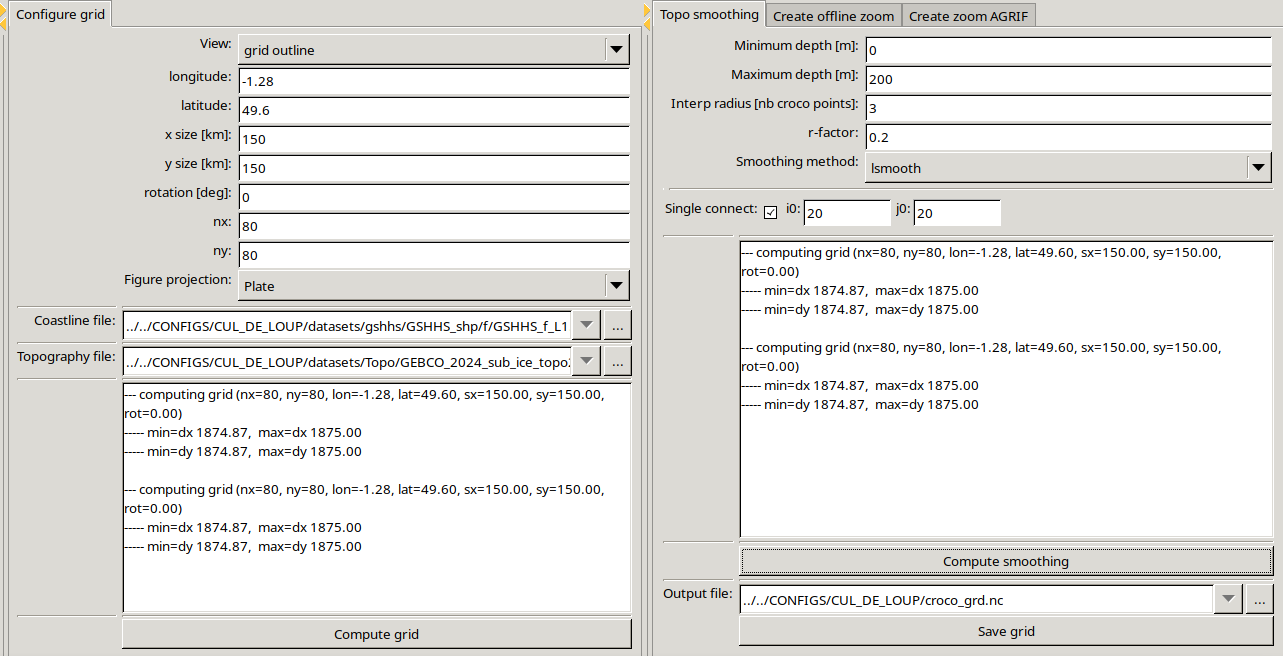
\includegraphics[scale=0.4]{../images/makegrid/parameters_main.png}
        
        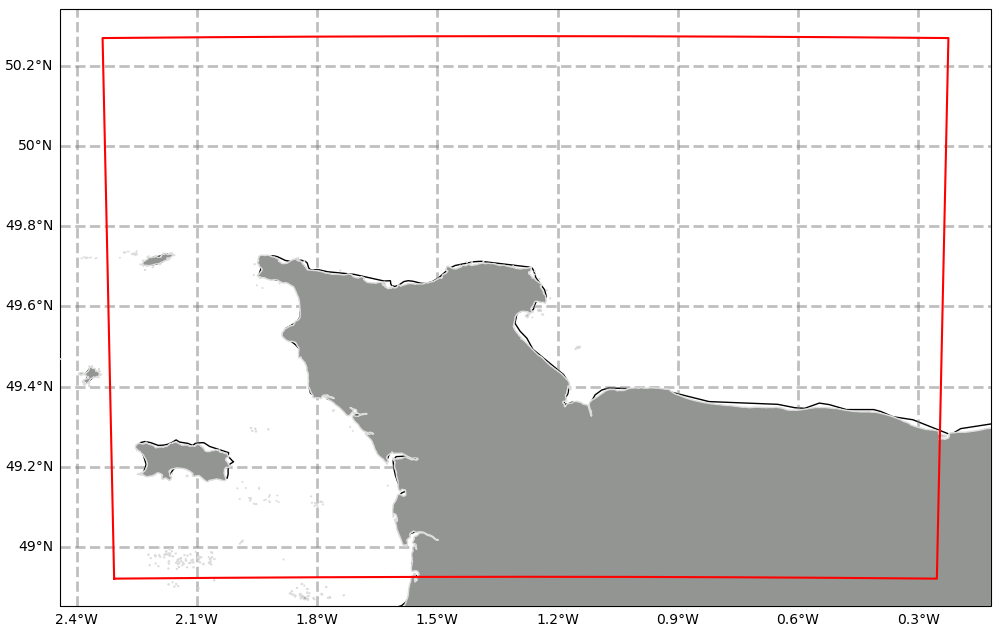
\includegraphics[scale=0.2]{../images/makegrid/config_main.png}
        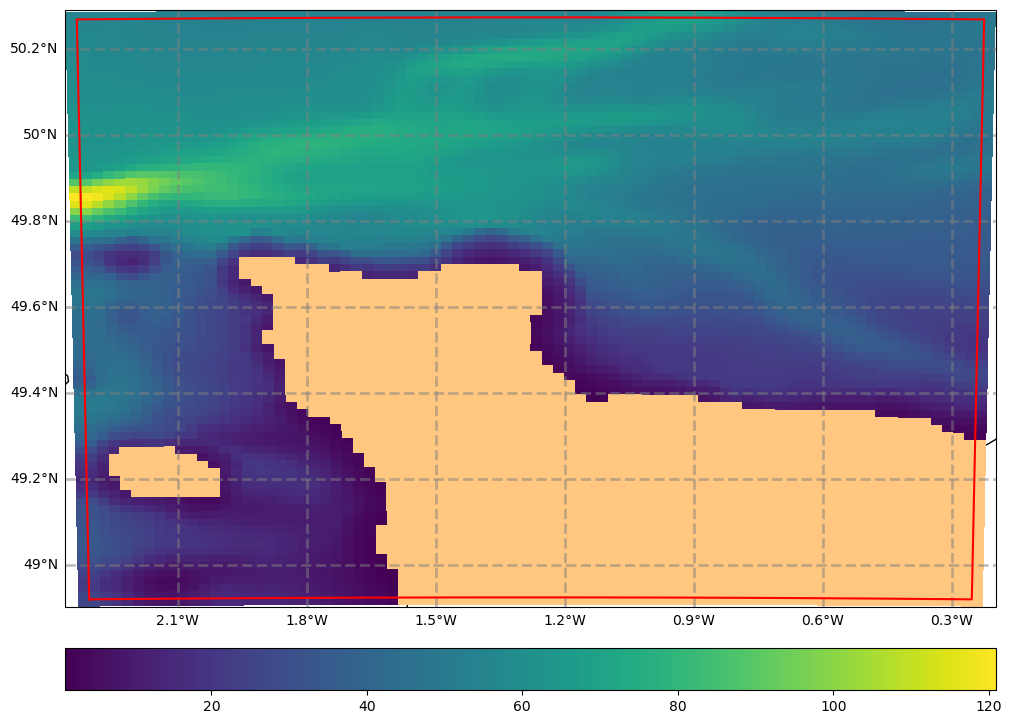
\includegraphics[scale=0.2]{../images/makegrid/ismooth_main.png}
        \caption{Caption.}
        \label{make_grid_main}
    \end{center}
\end{figure}


\textbf{make\_ini.py}

L'entête du code \textit{make\_ini.py} doit être adaptée aux paramètres choisis et à l'emplacement des données.

\begin{codeEnv}{\textbf{modifications utilisateur·ice de \textit{make\_ini.py}}}
    \begin{lstlisting}[language=python]
        #--- USER CHANGES ---------------------------------------------------------
        
        # Dates
        # starting date
        Yini, Mini, Dini, Hini  = '2013', '11', '28', '01'  # Month and days need to be
        #       2-digits format reference time (default = ini time)
        Yorig, Morig, Dorig= '1970', '01', '01'  # Month and days need to be
        #       2-digits format
        
        # Input data information and formating
        inputdata = 'copernicus'  # Input data dictionnary as defined in the
        #       Readers/ibc_reader.py
        input_dir = 'PATH-TO-CONFIGS/CONFIGS/CONFIG-NAME/dataset/Ini/'
        input_prefix='copernicus_marine_data'
        #input_file  = f'{input_dir}{input_prefix}Y{Yini}M{Mini}.cdf'
        input_file  = f'{input_dir}{input_prefix}.nc'
        multi_files=False  # If variables are in different netcdf
        if multi_files:  # Mutiple files
        input_file = { 'ssh'  : input_dir + input_prefix + 'ETAN.Y2013M01.nc',\
            'temp' : input_dir + input_prefix + 'THETA.Y2013M01.nc',\
            'salt' : input_dir + input_prefix + 'SALT.Y2013M01.nc',\
            'u'    : input_dir + input_prefix + 'EVEL.Y2013M01.nc',\
            'v'    : input_dir + input_prefix + 'NVEL.Y2013M01.nc'\
        }
        
        # time index to use in the file
        tndx = 0
        
        # default value to consider a z-level fine to be used
        Nzgoodmin = 4
        
        # tracers
        tracers = ['temp','salt']
        
        # CROCO grid informations
        croco_dir = 'PATH-TO-CONFIGS/CONFIGS/CONFIG-NAME/preproOUTPUT/'
        croco_grd = 'croco_grd.nc'
        sigma_params = dict(theta_s=7, theta_b=2, N=32, hc=200)  # Vertical streching,
        #       sig_surf/sig_bot/ nb level/critical depth
        
        # Ini file informations
        ini_filename = 'croco_ini.nc'  # output will be put in croco_dir by default
        
        # Conserv OGCM transport option
        conserv=1  # Correct the horizontal transport i.e. remove the integrated
        #       transport and add the OGCM transport
        
        #--- END USER CHANGES -----------------------------------------------------
        
    \end{lstlisting}
\end{codeEnv}

Pour que les codes d'initialisation et de conditions aux limites fonctionnent correctement, il convient de s'assurer que le code \textit{Readers/ibc\_reader.py} soit correctement rempli.  Ici, on ajoute le dictionnaire pour les données copernicus.

\begin{codeEnv}{\textbf{modifications de \textit{Readers/ibc\_reader.py}}}
    \begin{lstlisting}[language=python]
        # ajouter dans  la fonction lookvar(input):
        # avant la ligne "else:" (vers la ligne 55)
        
        elif input == 'copernicus':
        dico={ 'depth':'depth',\
            'lonr':'longitude','lonu':'longitude','lonv':'longitude',\
            'latr':'latitude','latu':'latitude','latv':'latitude',\
            'ssh':'zos',\
            'temp':'thetao',\
            'salt':'so',\
            'u': 'uo',\
            'v': 'vo',\
            'time': 'time',\
            'time_dim':'time'\
        }
    \end{lstlisting}
\end{codeEnv}

\textbf{make\_bry.py}

L'entête du code \textit{make\_bry.py} doit être adaptée aux paramètres choisis et à l'emplacement des données.

\begin{codeEnv}{\textbf{modifications utilisateur·ice de \textit{make\_bry.py}}}
    \begin{lstlisting}[language=python]
        #--- USER CHANGES ---------------------------------------------------------
        
        # Dates
        Yorig, Morig, Dorig = '1970', '01', '01'  # origin of time as: days since
        #       Yorig-Morig-Dorig-00h00
        Ystart, Mstart, Dstart, Hstart = '2013', '11', '28', '01'  # Starting month
        Yend, Mend, Dend, Hend  = '2014','03', '01', '01'  # Ending month
        
        # Input data information and formating
        inputdata = 'copernicus'  # Input data dictionnary as defined in the
        #       Readers/ibc_reader.py
        input_dir = 'PATH-TO-CONFIGS/CONFIGS/CONFIG-NAME/datasets/Bry/'
        input_prefix = 'copernicus_marine_data'  # Please use * to include all files
        multi_files = False
        if multi_files: # Multiple data files. Time is read in ssh file
        input_file = {'ssh':sorted(glob.glob(input_dir+input_prefix+'ETAN.*.nc')),\
            'temp':sorted(glob.glob(input_dir+input_prefix+'THETA.*.nc')),\
            'salt':sorted(glob.glob(input_dir+input_prefix+'SALT.*.nc')),\
            'u':sorted(glob.glob(input_dir+input_prefix+'EVEL.*.nc')),\
            'v':sorted(glob.glob(input_dir+input_prefix+'NVEL.*.nc'))\
        }
        else:  # glob all files
        input_file  = sorted(glob.glob(input_dir + input_prefix))
        
        # default value to consider a z-level fine to be used
        Nzgoodmin = 4
        
        # Tracers
        tracers = ['temp', 'salt']
        
        # CROCO grid informations
        croco_dir = 'PATH-TO-CONFIGS/CONFIGS/CONFIG-NAME/preproOUTPUT/'
        croco_grd = 'croco_grd.nc'
        sigma_params = dict(theta_s=7, theta_b=2, N=32, hc=200)  # Vertical streching,
        #       sig_surf/sig_bot/ nb level/critical depth
        
        # Bry file informations
        bry_filename = 'croco_bry.nc'  # output will be put in croco_dir by default
        obc_dict = dict(south=1, west=1, east=1, north=1) # open boundaries
        #       (1=open , [S W E N])
        output_file_format = "FULL"  # How outputs are spit (MONTHLY,YEARLY,FULL)
        cycle_bry = 0.
        
        # Conserv OGCM transport option
        conserv=1  # Correct the horizontal transport i.e. remove the integrated
        #       tranport and add the OGCM transport
        
        #--- END USER CHANGES -----------------------------------------------------
    \end{lstlisting}
\end{codeEnv}

Quelques modifications doivent aussi être effectuées dans le corps du code comme décrit ci-dessous.

\begin{codeEnv}{\textbf{modifications supplémentaires de \textit{make\_bry.py}}}
    \begin{lstlisting}[language=python]
        # ligne 111
        # ORIGINAL :
        start_date = Ystart+Mstart+'01'+'12'  # defaut start day is 1st
        # NOUVEAU :
        start_date = Ystart+Mstart+Dstart+Hstart  # defaut start day is 1st
        
        # ligne 119
        # ORIGINAL :
        dtenddt = plt.datetime.datetime(int(Yend),int(Mend),1,12) \
        # NOUVEAU :
        dtenddt = plt.datetime.datetime(int(Yend),int(Mend),int(Dend),int(Hend)) \
    \end{lstlisting}
\end{codeEnv}


\textbf{make\_blk\_interpol.py}

L'entête du code \textit{make\_blk\_interpol.py} doit être adaptée aux paramètres choisis et à l'emplacement des données.

le code est présenté en annexes, ajouter un schéma du fonctionnement du code.

schéma descriptif du fonctionnement du code [FIGURE À FAIRE]

\begin{codeEnv}{\textbf{modifications utilisateur·ice de \textit{make\_blk\_interpol.py}}}
    \begin{lstlisting}[language=python]
        ############################ User changes ############################
        # don't change de left part of the dictionnary (keys)
        
        INPUT_PARAM = {	"lon": "longitude",
            "lat": "latitude",
            "time": "valid_time",
            "Tair": "t2m",
            "HumiditeRelat": "RH",
            "PrecipitationRate": "avg_tprate",
            "WindSpeed": "si10",
            "NetLWRadiation": "avg_snlwrf",
            "DownwardLWRadiation": "avg_sdlwrf",
            "SWRadiation": "avg_snswrf",
            "UStress": "avg_iews",
            "VStress": "avg_inss",
            "UWind": "u10",
            "VWind": "v10"
        }
        
        INPUT = {
            "dir": "PATH-TO-CONFIGS/CONFIGS/CONFIG-NAME/datasets/Bulk/",
            "file": 'cpernicus_atmospheric_data.nc',
            "param": INPUT_PARAM
        }
        
        output_param = {"time": "bulk_time",
            "Tair": "tair",
            "HumiditeRelat": "rhum",
            "PrecipitationRate": "prate",
            "WindSpeed": "wspd",
            "NetLWRadiation": "radlw",
            "DownwardLWRadiation": "radlw_in",
            "SWRadiation": "radsw",
            "UStress": "sustr",
            "VStress": "svstr",
            "UWind": "uwnd",
            "VWind": "vwnd"
        }
        
        OUTPUT = {	"dir": "PATH-TO-CONFIGS/CONFIGS/CONFIG-NAME/preproOUTPUT/",
            "file": 'croco_blk.nc',
            "param": output_param
        }
        
        NB_VOISINS = 8
        
        sigma_params = dict(theta_s=0, theta_b=0, N=1, hc=1)
        
        ########################## END User changes ##########################
    \end{lstlisting}
\end{codeEnv}

\textbf{make\_frc\_tide.py}

L'entête du code \textit{make\_frc\_tide.py} doit être adaptée aux paramètres choisis et à l'emplacement des données.

le code complet est présenté en annexes, ajouter un schéma du fonctionnement du code.

schéma descriptif du fonctionnement du code [FIGURE À FAIRE]

\begin{codeEnv}{\textbf{modifications utilisateur·ice de \textit{make\_frc\_tide.py}}}
    \begin{lstlisting}[language=python]
        # sera modifie pour que ce soit des disctionnaires si on le veut dans le rapport
        
        ############################ User changes ############################
        
        Correction_uv = False
        tides = ['M2','S2','N2','K2','K1','O1','P1','Q1','Mf','Mm']
        
        grid_dir = "PATH-TO-CONFIGS/CONFIGS/CONFIG-NAME/preproOUTPUT/"
        grid_name = "croco_grd.nc"
        #grid_param = ["lon_rho", "lat_rho", "lon_u", "lat_u", "lon_v", "lat_v"]
        grid_param = ["lon_rho", "lat_rho", "lon_rho", "lat_rho", "lon_rho", "lat_rho"]
        print("\n grid param : \n", grid_param)
        grid_param_meaning = ["lonH", "latH", "lonU", "latU", "lonV", "latV"]  # don't change this order
        
        input_dir = "PATH-TO-CONFIGS/CONFIGS/CONFIG-NAME/datasets/Bry/AVISO/"
        TPXO_or_AVISO = True  # 0 or False for TPXO    and    1 or True for AVISO
        multi_file = True  # 0 or False if monofile   and   1 or True if multifile
        name_is_tide = True  # if the files names ar tide_name.nc
        #input_file_name = 'FES2014*.nc'
        input_file_name = [ "ocean_tide_extrapolated/",
        "eastward_velocity/",
        "northward_velocity/"
        ]
        prefix = ""
        sufix = ".nc"
        if name_is_tide :  # generate automatically the multifile names
        path_names = copy.copy(input_file_name)
        for i,path in enumerate(path_names):
        input_file_name[i] = []
        for tide in tides:
        input_file_name[i].append(path + prefix + tide.lower() + sufix)
        input_file_name = np.array(input_file_name)
        print("\ninput directory :\n", input_dir)
        print("\ninput files : \n", input_file_name)
        
        input_param_names = [   ["lat", "lon", "phase", "amplitude"],
        ["lat", "lon", "Ug", "Ua"],
        ["lat", "lon", "Vg", "Va"],
        ]
        print("\n input param names : \n", input_param_names)
        input_param_meaning =   [   ["latH", "lonH", "phaseH", "amplitudeH"],
        ["latU", "lonU", "phaseU", "amplitudeU"],
        ["latV", "lonV", "phaseV", "amplitudeV"],
        ]  # keep same names as grid_param_meaning
        print("\n input param meaning : \n", input_param_meaning)
        
        output_dir = "../CONFIGS/CUL_DE_LOUP/GRIDS/"
        output_file_name = 'croco_frc.nc'
        output_param = ["tide_period", "tide_Ephase", "tide_Eamp",
        "tide_Cmin", "tide_Cmax", "tide_Cangle", "tide_Cphase"]  # don't change the order
        
        tide_param_path="prepro/Modules/tides.txt"
        
        NB_VOISINS = 8
        
        ########################## END User changes ##########################
    \end{lstlisting}
\end{codeEnv}

\subsubsection{Détail des processus du modèle}
schéma détaillé de la marche à suivre pour faire fonctionner le modèle à partir des fichiers du pre-processing.

\subsection{Le modèle "anse du Cul-de-Loup"}

Grosse partie dans laquelle il va falloir expliquer les différentes étapes de mis en place du modèle ADCL

détailler les paramètres choisis

\subsection{Mesures de terrain - Le projet PROTEC}

Pour moi: quelques mots sur les données disponibles pour comparer les résultats modèle avec des mesures de terrain (cf Discussion)



\end{document}

